\section{Introduction}
\begin{frame}{Introduction}
  \begin{itemize}
  \item There is the need to develop software to solve systems with renewables, and hence, power converters. 
  \item It is paramount to not exceed the current limitations of converters.
  \item Converters may have to operate under saturated conditions, especially during short-circuit faults.
  \end{itemize}

  Some solutions to solve this problem are:
  \begin{itemize}
    \item Inject a precalculated current in short-circuit calculations, as in PSSe or PowerFactory. The angle is unknown and the dependency on the voltage is not considered.
    \item Conduct a dynamic simulation.
  \end{itemize}
  However, it is preferable to add a new set of equations and bus types. The simulation becomes more precise and significantly faster. 

  The presentation covers the modelling, formulation, an overview of the solver, and results for the Texas 2000-bus synthetic grid.

\end{frame}


% ------------------
\section{Modelling}

\subsection{Bus types}
\begin{frame}{Traditional power flow}
Buses are grouped under three categories:

\begin{table}[!htb]\centering
  \caption{Types of bus in traditional systems.}
  \begin{tabular}{cccc}
    \hline
    \textbf{Variables} & \textbf{Slack} & \textbf{PQ} & \textbf{PV} \\
    \hline
    \hline
    \textbf{Inputs} & $\delta, V$ & $P, Q$ & $P, V$ \\
    \textbf{Unknowns} & $P, Q$ & $\delta, V$ & $\delta, Q$ \\
    \hline
  \end{tabular}
  \label{tab:3bus}
\end{table}
A system of $2(n-1)$ equations is derived, being $n$ the number of buses. With the Newton-Raphson method, in polar form, we have a system of size $2n_{pq} + n_{pv}$:

\begin{equation}
  - \begin{pmatrix}
    \bm{\Delta P} \\
    \bm{\Delta Q} \\
   \end{pmatrix} = 
  \begin{pmatrix}
    \bm{J1} & \bm{J2} \\
    \bm{J3} & \bm{J4} \\
  \end{pmatrix}
  \cdot
  \begin{pmatrix}
    \bm{\Delta \delta} \\
    \bm{\Delta V} \\
  \end{pmatrix} .
\end{equation}
\end{frame}

% \begin{frame}{New paradigm}
%   Adding Voltage Source Converters (VSCs) yields a new paradigm. 

%   \begin{itemize}
%     \item The current $I$ may have to be controlled to not exceed the limitations.
%     \item The set of variables grows: $\delta, V, P, Q, I$.
%   \end{itemize}
%   Not only we can have $PQ$ and $PV$ buses, but also $PI$, $QI$ and $VI$ buses for instance. The general system becomes:
% \begin{equation}
%   - \begin{pmatrix}
%     \bm{\Delta P} \\
%     \bm{\Delta Q} \\
%     \bm{\Delta I} \\
%    \end{pmatrix} = 
%   \begin{pmatrix}
%     \bm{J1} & \bm{J2} \\
%     \bm{J3} & \bm{J4} \\
%     \bm{J5} & \bm{J6} \\
%   \end{pmatrix}
%   \cdot
%   \begin{pmatrix}
%     \bm{\Delta \delta} \\
%     \bm{\Delta V} \\
%   \end{pmatrix},
% \end{equation}
% where $\bm{J5} = \dfrac{\bm{dI}}{\bm{d\delta}}$ and $\bm{J6} = \dfrac{\bm{dI}}{\bm{dV}}$.

% \end{frame}

% \begin{frame}{Conventional Approach to Model VSCs}
% In PSSE, VSCs can be modeled with two options following IEC 60909 standard for short-circuit calculation:
%   \begin{itemize}
% 	\item Modeled as FACTS, which is ignored or modeled as a load admittance during the fault. 
% 	\item Modeled as converter-interfaced renewable generation, which is expressed as Norton equivalent for short-circuit calculation.
% \end{itemize} 	

% Both options failed to include the converter control and potential current-saturation correctly.

% \end{frame}



% \begin{frame}{Our Modeling for Short-Circuit Calculation}

% \begin{table}[!htb]
%   \caption{Modeling of loads, synchronous machines and VSCs for Short-Circuit Calculation.}
% 	\begin{center}
% 		\begin{tabular}{m{2cm}<{\centering}|m{4cm}<{\centering}m{4cm}<{\centering}}
% 			\toprule
% 			Type of elements & Normal Operation analysis & Short-Circuit Calculation	\\
% 			\midrule
% 			Load & PQ node & Constant impedance \\
% 			\hline
% 			Synchronous Machine & PQ/PV node & Thévenin equivalent\\
% 			\hline
% 			VSC & Depending on control mode and various current-saturation states & Depending on control mode and various current-saturation states\\
% 			\bottomrule
% 		\end{tabular}
% 	\end{center}
% \end{table}	

% \end{frame}

% \subsection{VSC states}
% \begin{frame}{VSC states}
%   We consider that VSCs can operate in the following modes:
% \begin{table}[!htb]\centering
%   \caption{Operating states of the converters in grid-following mode.}
%   \begin{tabular}{ccc}
%     \hline
%     & \textbf{PQ} & \textbf{PV} \\
%     \hline
%     \textbf{USS} & $P$, $Q$ & $P$, $V$ \\
%     \textbf{PSS} & $Q$, $I_{max}$ & $V$, $I_{max}$ \\
%     \textbf{FSS} & $P=0$, $I_{max}$ & $P=0$, $I_{max}$ \\
%     \textbf{DIS} & $P=0$, $Q=0$ & $P=0$, $Q=0$ \\
%     \hline
%   \end{tabular}
%   \label{tab:convs1}
% \end{table}

% \begin{itemize}
%   \item USS: unsaturated, just like a traditional bus.
%   \item PSS: partially saturated, current limits are reached.
%   \item FSS: fully saturated, more severe than PSS.
%   \item DIS: disconnected due to abnormal conditions.
% \end{itemize}

% \end{frame}

% \section{Formulation}
% \subsection{Residuals}
% \begin{frame}{Residuals}
%   \begin{itemize}
%     \item Calculated in matrix form:
%   \end{itemize}

% \begin{equation}
%   {\Delta f_P} = - {P_{set}} + \Re([{V}]{Y}^*{V}^* - [V]I^*_l),
% \end{equation}
% \begin{equation}
%   {\Delta f_Q} = - {Q_{set}} + \Im([{V}]{Y}^*{V}^* - [V]I^*_l),
% \end{equation}
% \begin{equation}
%   {\Delta f_{I^2}} =  - {I_{c,max}}^2 + ({Y}{V} - [{V}^*]^{-1} {S}^* - {I_l}) \cdot ({Y}{V} - [{V}^*]^{-1} {S}^* - {I_l})^*.
% \end{equation}


% \begin{figure}[!htb]\centering
%   \begin{circuitikz}[european]
%     \draw[line width=0.1cm] (0,0.1) to [short] (0,-0.9);
%     \draw (0,-0.4) to [/tikz/circuitikz/bipoles/length=25pt, R, l=$\underline{Y}_{ir}$] (3,-0.4);

%     \draw (-1.0,-1) to [short, i=$\underline{S}_i$] (-1.0,-0.9);
%     \draw (-1.0,-0.9) to [short] (-1.0,-0.7);
%     \draw (-1.0,-1.0) to [voltage source, /tikz/circuitikz/bipoles/length=25pt] (-1.0,-2.0);
%     \draw (0,-0.7) to [short] (-1.0,-0.7);
%     \draw (-1.2,-2.0) to [short] (-0.8,-2.0);

%     \draw (1.0,-2.0) to [american current source, /tikz/circuitikz/bipoles/length=25pt] (1.0,-1.0);
%     \draw (1.0,-1) to [short, i_=$\underline{I}_{li}$] (1.0,-0.9);
%     \draw (1.0,-1.0) to [short] (1.0,-0.7);
%     \draw (1.0,-0.7) to [short] (0,-0.7);
%     \draw (1.2,-2.0) to [short] (0.8,-2.0);
    
%     \draw (-2.3,-0.4) to [sdcac, /tikz/circuitikz/bipoles/length=25pt] (-1.7,-0.4);
%     \draw (-1.7,-0.4) to [short, i=$\underline{I}_{ci}$] (-0.0, -0.4);

%     \draw (0,-1.0) to [short] (0,-0.9);
%     \draw (0,-1.0) to [/tikz/circuitikz/bipoles/length=25pt, R, l=$\underline{Y}_{ii}$] (0,-2.0);
%     \draw (0.2,-2.0) to [short] (-0.2,-2.0);

%     \node[] at (0,0.3) {$\underline{V}_i$};

%     \draw[line width=0.1cm] (3,-0.15) to [short] (3,-0.65);

%     \node[] at (3,0.1) {$\underline{V}_r$};

%   \end{circuitikz}
%   \caption{Generic bus with a power converter.}
%   \label{fig:rep1}
% \end{figure}

% \end{frame}

% \subsection{Jacobian}
% \begin{frame}{Jacobian matrices}
%   \begin{itemize}
%     \item The Jacobian is the central part of the Newton-Raphson (NR).
%     \item Crucial to calculate it fast $\rightarrow$ avoid loops, use matrices, Matpower way.
%   \end{itemize}

% \begin{equation}
%   J1 = \dfrac{dP}{d\delta} = \Re \bigl(j[V]([YV]^* - Y^*[V]^* - [I_l]^*) \bigr),
% \end{equation}
% \begin{equation}
%   J2 = \dfrac{dP}{d\nu} = \Re \bigl([V]([YV]^* + Y^*[V]^* - [I_l]^*)[\nu]^{-1} \bigr),
% \end{equation}
% \begin{equation}
%   J3 = \dfrac{dQ}{d\delta} = \Im \bigl(j[V]([YV]^* - Y^*[V]^* - [I_l]^*) \bigr),
% \end{equation}
% \begin{equation}
%   J4 = \dfrac{dQ}{d\nu} = \Im \bigl([V]([YV]^* + Y^*[V]^* - [I_l]^*)[\nu]^{-1} \bigr).
% \end{equation}

% \end{frame}

% \begin{frame}{Jacobian matrices}
%   For the squared absolute value of the current:

% \begin{equation}
%   J5 = \frac{dI^2}{d\delta} = [{I_c}]\left(\frac{d {I_c}}{d {\delta}}\right)^* + [{I_c}]^* \left(\frac{d {I_c}}{d {\delta}}\right) = 2\Re\left( [{I_c}]\left(\frac{d {I_c}}{d {\delta}}\right)^* \right),
% \end{equation}
% \begin{equation}
%   J6 = \frac{dI^2}{d\nu} = [{I_c}]\left(\frac{d {I_c}}{d {\nu}}\right)^* + [{I_c}]^* \left(\frac{d {I_c}}{d {\nu}}\right) = 2\Re\left( [{I_c}]\left(\frac{d {I_c}}{d {\nu}}\right)^* \right), 
% \end{equation}
% \begin{equation}
%   \frac{d {I_c}}{d {\delta}} = j({Y}[{V}] - [{S}]^*[{V}^*]^{-1}),
% \end{equation}
% \begin{equation}
%   \frac{d {I_c}}{d {\nu}} = ([{S}]^*[{V}^*]^{-1} + {Y}[{V}])[{\nu}]^{-1},
% \end{equation}
% \begin{equation}
%   [I_c] = [({Y}{V} - [{V}^*]^{-1} {S}^* - {I_l})].
% \end{equation}

% \end{frame}

% \section{Solver}


% \subsection{Algorithm overview}
% \begin{frame}{General view of the algorithm}

% \RestyleAlgo{ruled}

% \begin{algorithm}[H]
% \caption{Full solver algorithm}
% \KwData{\texttt{snap}, \texttt{states}, $\epsilon$}
% \KwResult{Solved system in \texttt{snap}}
% \texttt{success} \gets \texttt{False}\;

% \texttt{states\_old} \gets \texttt{states}\;

% Initialize objects in \texttt{snap}\

% \While {\texttt{success}=\texttt{False} or \texttt{states} $\neq$ \texttt{states\_old}}{ 
% \texttt{states\_old} \gets \texttt{states}\;

% \While {$\max(\bm{\Delta f}) > \epsilon$}{
%     \texttt{snap} = \texttt{inner\_loop(snap)}
% }
% \texttt{success} \gets \texttt{True}\;

% \texttt{states} \gets \texttt{update\_states(snap)}

% }
% \label{alg:1}
% \end{algorithm}
% \end{frame}


% \begin{frame}{Solver diagram}
%   \begin{figure}\tiny
%   \incfig{scheme3}
%   \caption{Scheme of the full algorithm.}
%   \label{fig:scheme2}
%   \end{figure}
% \end{frame}



% \begin{frame}{Update of states}

% In PQ mode:
% \begin{equation}
%     s = \begin{cases}
%         % \text{USS} & \text{if } |p_{ref}+jq_{ref}|\leq ui_{max} \\
%         % \text{PSS} & \text{if } q_{ref} \leq ui_{max} < |p_{ref} + jq_{ref}| \\
%         % \text{FSS} & \text{if } ui_{max} < q_{ref} \\
%         % \text{DIS} & \text{if } u<u_{min} \text{ or } u>u_{max} \\
%         \text{USS} & \text{if } |p + jq|\leq ui_{max} \\
%         \text{PSS} & \text{if } q_{ref} \leq ui_{max} < |p + jq| \\
%         \text{FSS} & \text{if } ui_{max} < q_{ref} \\
%         \text{DIS} & \text{if } u<u_{min} \text{ or } u>u_{max} \\
%     \end{cases}
% \end{equation}

% In PV mode:
% % \begin{equation}
% %     s = \begin{cases}
% %         \text{USS} & \text{if } |p+jq|\leq ui_{max} \\
% %         \text{PSS} & \text{if } q_{max} \leq ui_{max} < |p+jq| \\
% %         \text{FSS} & \text{if } ui_{max} < q_{max} \\
% %         \text{DIS} & \text{if } u<u_{min} \text{ or } u>u_{max} \\
% %     \end{cases}
% % \end{equation}

% \begin{figure}
%   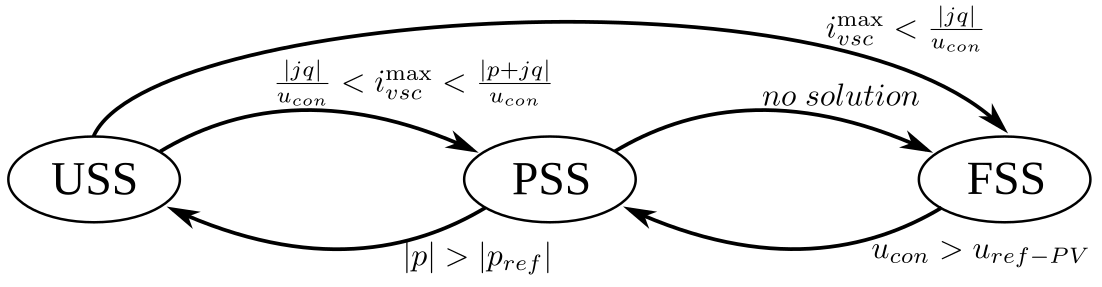
\includegraphics[width=10cm]{Data/pv3.png}
%   \caption{Heuristics to determine the states of PV VSCs.}
%   \label{fig:pv_state}
% \end{figure}

% \end{frame}

% \subsection{Hybrid solver}
% \begin{frame}{Hybrid solver}
%   \begin{itemize}
%     \item During faults, synchronous generators are modelled by a Thevenin equivalent and loads are treated as impedances. They are linear devices.
%     \item Converters may be saturated, an according to their states, they act as non-linear elements.
%     \item The hybrid solver combines linear devices with the non-linear converters.
%   \end{itemize}



%   \begin{columns}[c]
%     \begin{column}{0.4\textwidth}
% \begin{figure}[!htb]\tiny
%   \begin{circuitikz}[european]

%     \draw[line width=0.1cm] (0,0.4) to [short] (0,-0.4);
%     \draw[line width=0.1cm] (2,0.4) to [short] (2,-0.4);
%     \draw[line width=0.1cm] (0.6,1.0) to [short] (1.4,1.0);
%     \draw[line width=0.1cm] (0.6,-1.0) to [short] (1.4,-1.0);

%     \draw (-0.4,0.0) to [sdcac, /tikz/circuitikz/bipoles/length=25pt] (-1.0,0.0);
%     \draw (-0.4,0.0) to [short] (0,0);

%     \draw (1.0,2.0) to [vsourcesin, /tikz/circuitikz/bipoles/length=25pt] (1.0,1.5);
%     \draw (1,1.0) to [short] (1,1.5);

%     \draw[-{Latex[scale=2.0]}] (1,-1.0) -- (1,-2);
%     \draw[-{Latex[scale=2.0]}] (2,-0.0) -- (3,-0);

%     \draw (0,0.2) to [short] (0.2,0.2);
%     \draw (0,-0.2) to [short] (0.2,-0.2);

%     \draw (0.8,1) to [short] (0.8,0.8);
%     \draw (1.2,1) to [short] (1.2,0.8);

%     \draw (0.8,-1) to [short] (0.8,-0.8);
%     \draw (1.2,-1) to [short] (1.2,-0.8);

%     \draw (2,0.2) to [short] (1.8,0.2);
%     \draw (2,-0.2) to [short] (1.8,-0.2);

%     \draw (0.2,0.2) to [short] (0.8,0.8);
%     \draw (1.2,0.8) to [short] (1.8,0.2);
%     \draw (1.8,-0.2) to [short] (1.2,-0.8);
%     \draw (0.8,-0.8) to [short] (0.2,-0.2);

%   \end{circuitikz}
%   \caption{Prefault conditions.}
% \end{figure}
% \end{column}

% \begin{column}{0.6\textwidth}
% \begin{figure}\tiny
%   \begin{circuitikz}[european, american currents]

%     \draw[line width=0.1cm] (0,0.4) to [short] (0,-0.4);
%     \draw[line width=0.1cm] (2,0.4) to [short] (2,-0.4);
%     \draw[line width=0.1cm] (0.6,1.0) to [short] (1.4,1.0);
%     \draw[line width=0.1cm] (0.6,-1.0) to [short] (1.4,-1.0);

%     % \draw (-1,-0.0) to [I, /tikz/circuitikz/bipoles/length=25pt] (-0.0,-0.0);
%     % \draw (-1.0,0.2) to [short] (-1.0,-0.2); 

%     \draw (-0.4,0.0) to [sdcac, /tikz/circuitikz/bipoles/length=25pt] (-1.0,0.0);
%     \draw (-0.4,0.0) to [short] (0,0);

%     \draw (1.0,2.5) to [vsourcesin, /tikz/circuitikz/bipoles/length=25pt] (1.0,2.0);
%     \draw (1,1.0) to [/tikz/circuitikz/bipoles/length=25pt, R] (1,2.0);
%     % \draw (0.8,2.0) to [short] (1.2,2.0); 

%     \draw (1,-1.0) to [/tikz/circuitikz/bipoles/length=25pt, R] (1,-2.0);
%     \draw (0.8,-2.0) to [short] (1.2,-2.0);

%     \draw (2,0) to [/tikz/circuitikz/bipoles/length=25pt, R] (3,0);
%     \draw (3,0.2) to [short] (3,-0.2);

%     \draw[red] (1.4,-1) to [short] (1.8,-1.0);
%     \draw[red] (1.8,-1.85) to [short] (1.8,-2);
%     \draw[red] (1.6,-2) to [short] (2.0,-2);

%     \draw[red] (1.8,-1) to [R, /tikz/circuitikz/bipoles/length=25pt, color=red] (1.8, -2);

%     \draw (0,0.2) to [short] (0.2,0.2);
%     \draw (0,-0.2) to [short] (0.2,-0.2);

%     \draw (0.8,1) to [short] (0.8,0.8);
%     \draw (1.2,1) to [short] (1.2,0.8);

%     \draw (0.8,-1) to [short] (0.8,-0.8);
%     \draw (1.2,-1) to [short] (1.2,-0.8);

%     \draw (2,0.2) to [short] (1.8,0.2);
%     \draw (2,-0.2) to [short] (1.8,-0.2);

%     \draw (0.2,0.2) to [short] (0.8,0.8);
%     \draw (1.2,0.8) to [short] (1.8,0.2);
%     \draw (1.8,-0.2) to [short] (1.2,-0.8);
%     \draw (0.8,-0.8) to [short] (0.2,-0.2);

%   \end{circuitikz}
%   \caption{System to solve with the fault.}
%   \label{fig:sync3}
% \end{figure}
% \end{column}

% \end{columns}

% \end{frame}


%   \begin{frame}{Hybrid solver steps}

% \begin{equation}
%   \underline{Z}_i = \frac{V_i^2}{\underline{S}_i^*},
%   \label{eq:loads}
% \end{equation}

% \begin{equation}
%   \underline{E}_i = \underline{V}_i + jX_{g,i} \underline{I}_{\text{inj},i},
%   \label{eq:syncs}
% \end{equation}


% \begin{enumerate}
%   \item Initialize the objects $\bm{Y}, \bm{V}, \bm{S}, \bm{I_l}$ and classify the buses: PQ, PV, PI, QI, VI. 
%   \item Solve the non-linear system of equations iteratively until a low error is reached. With this, the prefault solution is obtained.
%   \item Linearize loads with Equation \ref{eq:loads}, synchronous generators with their corresponding Thevenin equivalent (see Equation \ref{eq:syncs}), and modify $\bm{Y}$ to include the fault impedance. 
%   \item Solve the hybrid system formed by linear synchronous generators and loads and non-linear converters. Objects $\bm{Y}$, $\bm{V}$ and $\bm{S}$ are modified and the looping steps in Figure \ref{fig:scheme2} are followed.
% \end{enumerate}

%   \end{frame}




% \section{Results}
% \subsection{Case study}

% \begin{frame}{2000-bus ACTIVSg2000 system}

% \begin{figure}[!htb]\centering
% \incfig{texas2}
% \caption{Placement of the three converters in the system.}
% \label{fig:texas}
% \end{figure}

% \end{frame}


% \begin{frame}{VSC data}
%   % Table of VSCs
% The input data for the three converters is:
% \begin{table}[!htb]\centering\scriptsize
%   \caption{Input data of the converters.}
%   \begin{tabular}{ccccccccccc}
%     \hline
%     \textbf{bus} & \textbf{type} & \textbf{state} & \textbf{pref} & \textbf{qref} & \textbf{vref} & \textbf{imax} & \textbf{vmin} & \textbf{vmax} & \textbf{kisp} & \textbf{id0} \\
%     \hline
%     1001 & pq & USS & -5.0 & 3.026 & 1.0 & 7.0 & 0.05 & 1.3 & 1.0 & 3.026 \\
%     4023 & pq & USS & -1.0 & 0.973 & 1.0 & 2.0 & 0.05 & 1.3 & 1.0 & 0.973 \\
%     8073 & pq & USS & 6.0 & 1.458 & 1.0 & 8.0 & 0.05 & 1.3 & 1.0 & 1.458 \\
%     \hline
%     \hline
%   \end{tabular}
%   \label{tab:convs1}
% \end{table}

% Grid-support is activated:
% \begin{equation}
%   q = q_{ref} + i_{sp}v.
% \end{equation}

% \noindent where the grid-support current $i_{sp}$ is:
% \begin{equation}
% 	i_{sp}=k_{isp}(v_{ref}-v).
% \end{equation}

% \end{frame}

% \begin{frame}{Normal operating state}
%   % solution of the non-linear power flow

% \begin{table}[!htb]\centering\scriptsize
%   \caption{Power flow results for the converters under normal conditions.}
%   \begin{tabular}{cccccccc}
%     \hline
%     \textbf{VSC} & \textbf{State} & $|\bm{V}|$ & \bm{\delta} & $|\bm{I}|$ & $\bm{P}$ & $\bm{Q}$ & $|\bm{S}|$ \\
%     \hline
%     vsc1 & USS & 1.007349 & -40.792494 & 5.801736 & -5.000000 & 3.0260 & 5.844371 \\
%     vsc2 & USS & 1.005099 & -63.956569 & 1.388243 & -1.000000 & 0.9731 & 1.395322 \\
%     vsc3 & USS & 1.020098 & -48.630110 & 6.052952 & 6.000000 & 1.4580 & 6.174606 \\
%     \hline
%     \hline
%   \end{tabular}
%   \label{tab:convs1}
% \end{table}

% \begin{table}[!htb]\centering\scriptsize
%   \caption{Power flow results for the converters with $Z_f=0.002j$.}
%   \begin{tabular}{cccccccc}
%     \hline
%     \textbf{VSC} & \textbf{State} & $|\bm{V}|$ & \bm{\delta} & $|\bm{I}|$ & $\bm{P}$ & $\bm{Q}$ & $|\bm{S}|$ \\
%     \hline
%     vsc1 & FSS & 0.063301 & -14.157682 & 7.000000 & 0.000000 & 0.443108 & 0.443108 \\
%     vsc2 & USS & 0.999726 & -63.383639 & 1.395825 & -1.000000 & 0.973274 & 1.395443 \\
%     vsc3 & USS & 0.999718 & -46.170131 & 6.176412 & 6.000000 & 1.458281 & 6.174673 \\
%     \hline
%     \hline
%   \end{tabular}
%   \label{tab:convs2}
% \end{table}

% \begin{table}[!htb]\centering\scriptsize
%   \caption{Power flow results for the converters with $Z_f=0.05j$.}
%   \begin{tabular}{cccccccc}
%     \hline
%     \textbf{VSC} & \textbf{State} & $|\bm{V}|$ & \bm{\delta} & $|\bm{I}|$ & $\bm{P}$ & $\bm{Q}$ & $|\bm{S}|$ \\
%     \hline
%     vsc1 & PSS & 0.642317 & -34.196295 & 7.000000 & -3.100985 & 3.255756 & 4.496219 \\
%     vsc2 & USS & 1.005099 & -63.956569 & 1.388243 & -1.000000 & 0.969620 & 1.392897 \\
%     vsc3 & USS & 1.020098 & -48.630110 & 6.052952 & 6.000000 & 1.445348 & 6.171631 \\
%     \hline
%     \hline
%   \end{tabular}
%   \label{tab:convs3}
% \end{table}


%  \end{frame}

% \begin{frame}{Comparison with PSSE Short-Circuit Calculation Results}

% \begin{table}[!htb]\centering\scriptsize
% 	\caption{Comparison of Short-Circuit Calculation.}
% 	\begin{tabular}{cccc}
% 		\toprule
% 		\backslashbox{$i_{sc}$}{$\underline{z}_{sc}$} & Our Approach & PSSE-Converters as Generators & PSSE-Converters as FACTS \\
% 		\midrule
% 		$j0.05$ & 12.75 & 13.40 & 12.17 \\
% 		\hline
% 		$j0.002$ & 31.40 & 32.57 & 25.91 \\
% 		\bottomrule
% 	\end{tabular}
% 	\label{tab:comparison}
% \end{table}

% \end{frame}

% \begin{frame}{Validation with PSSE Simulation}
%   % 0.002j
% \begin{figure}
%   	\subfigure[VSC1 Power Injections]{
%     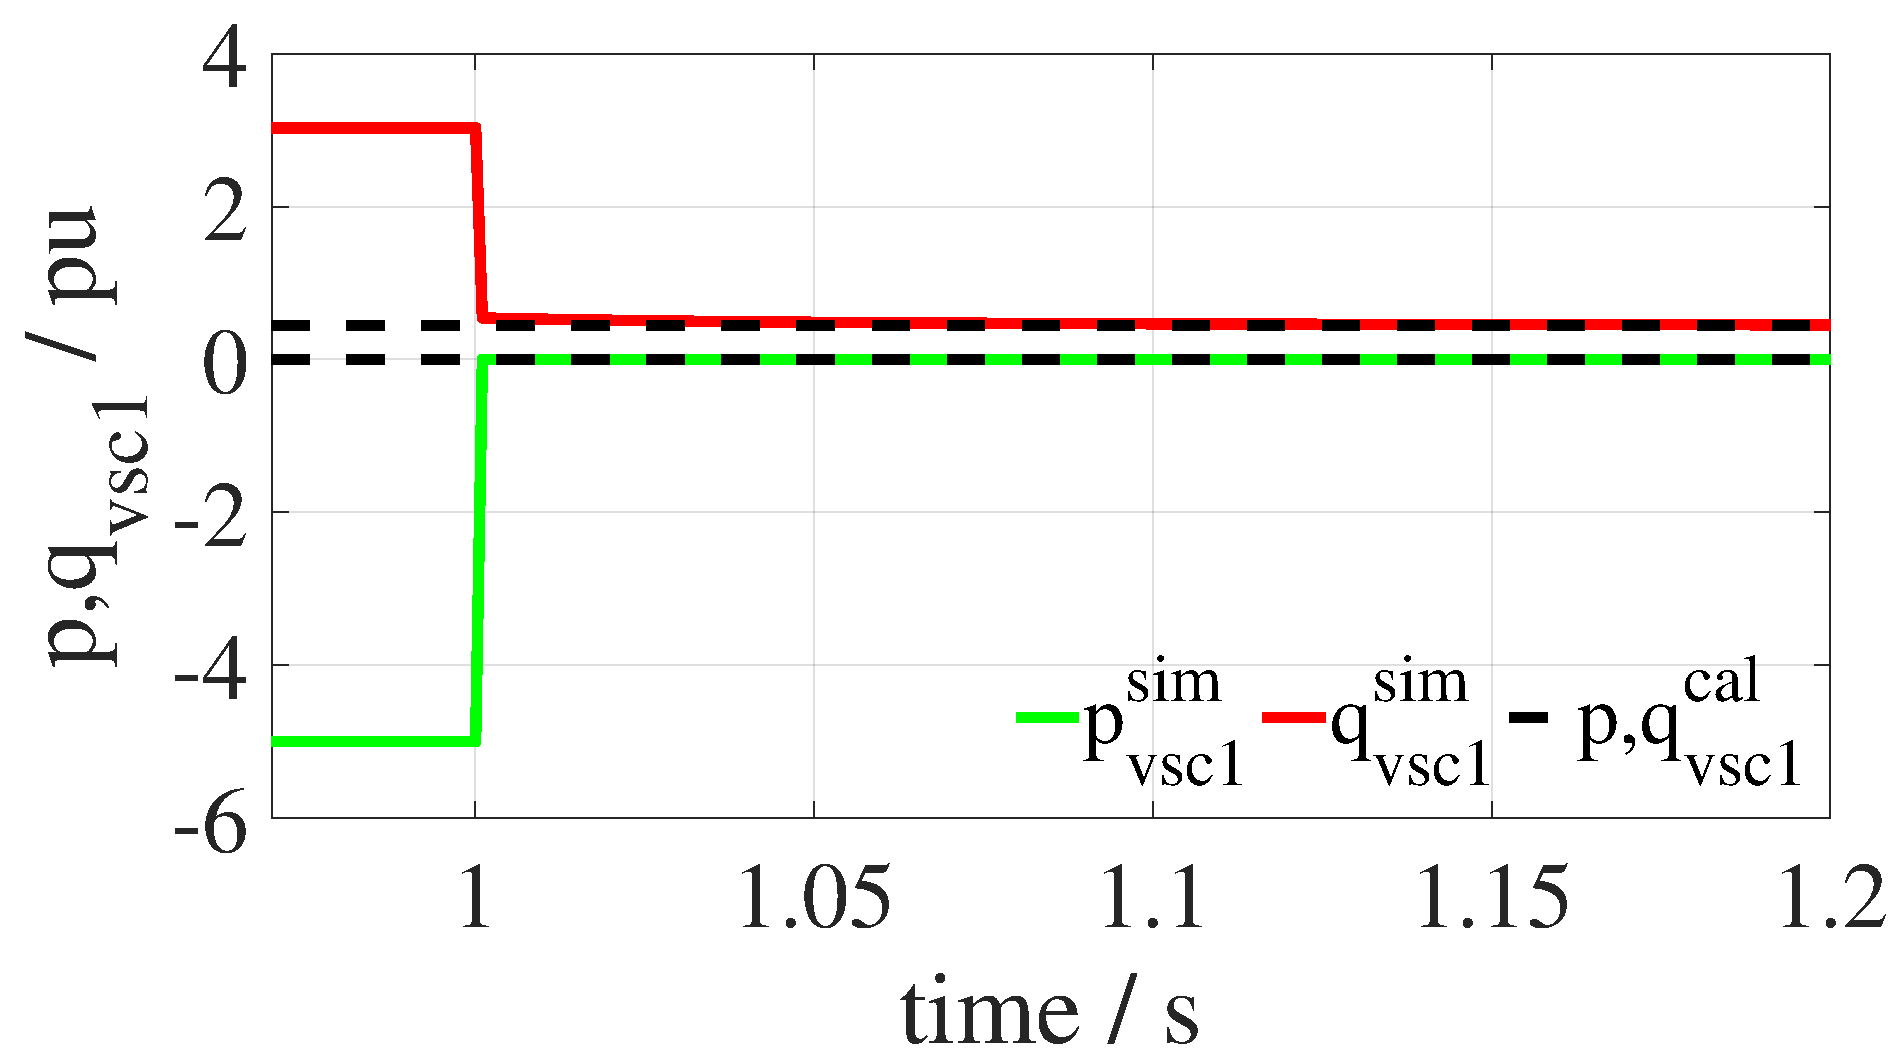
\includegraphics[width=4cm]{Data/Figure/psim_z0002.pdf}}
% 	\subfigure[Fault Voltage]{
%     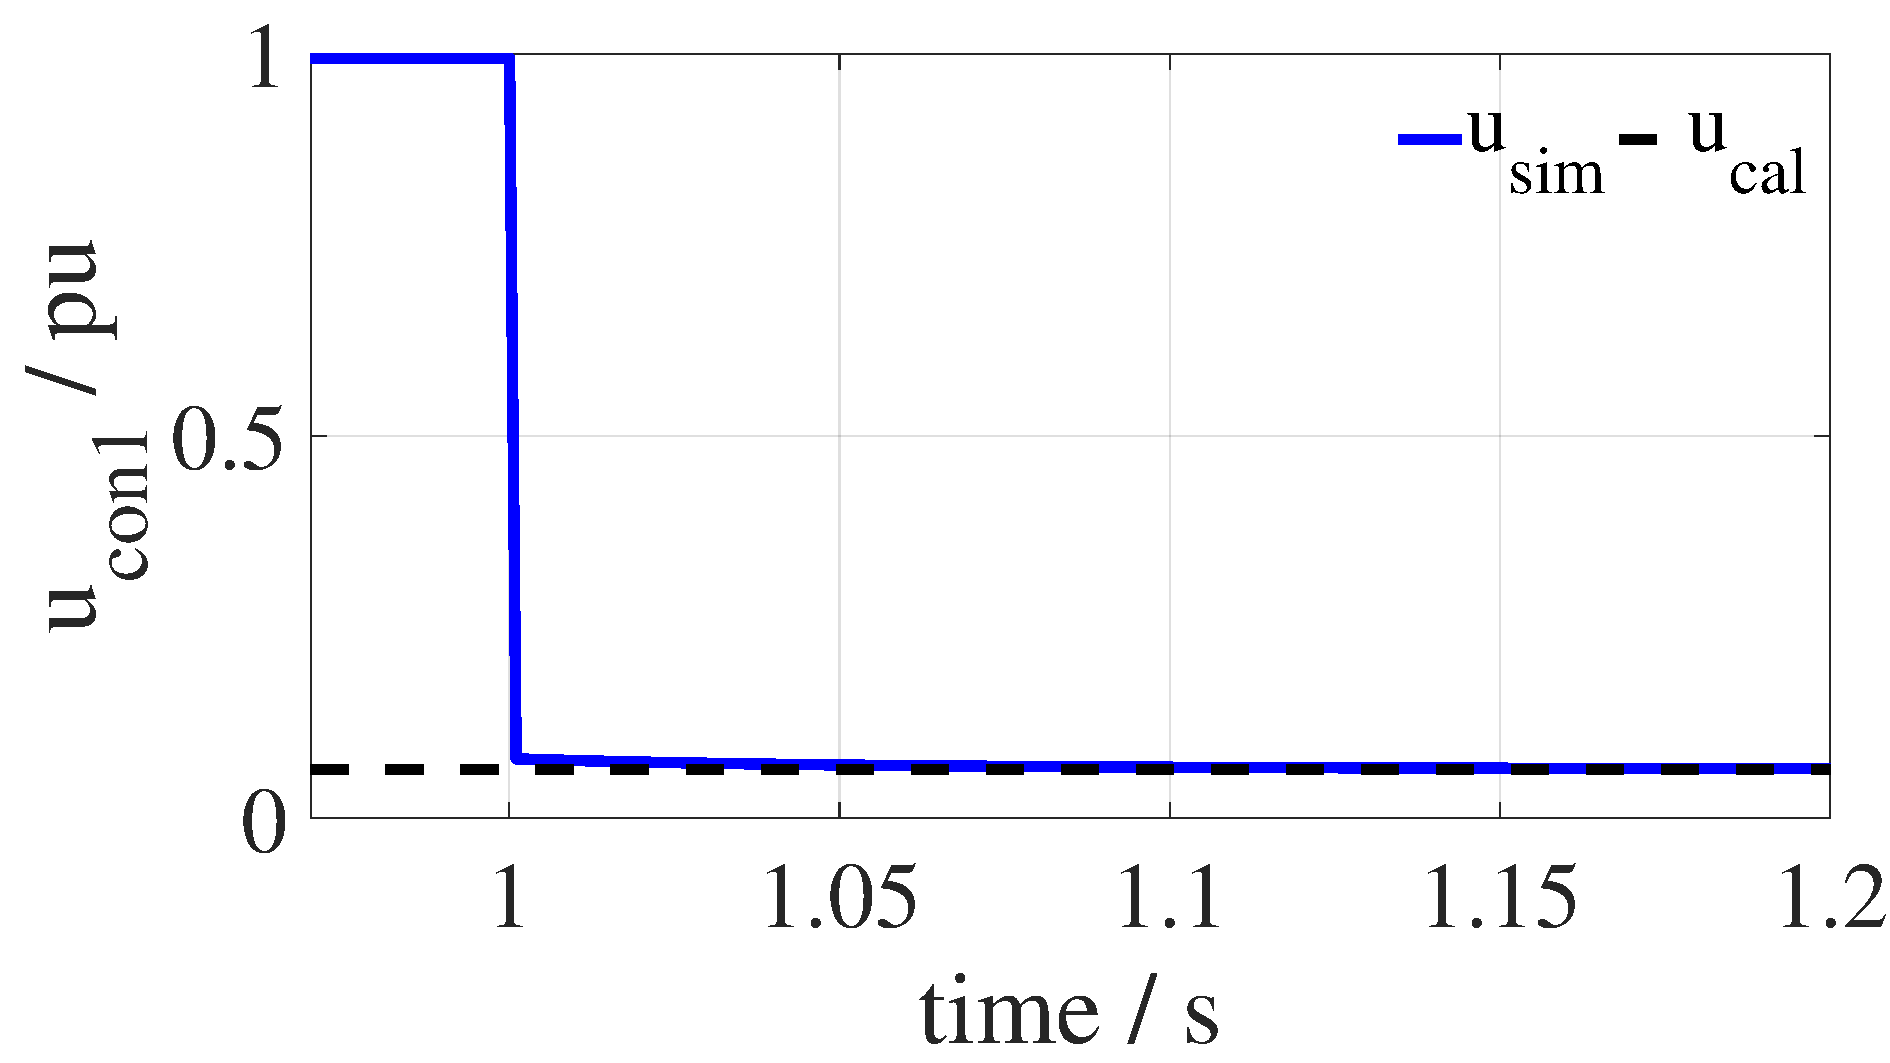
\includegraphics[width=4cm]{Data/Figure/usim_z0002.pdf}}
% 	\vskip -2mm
% 	\caption{Severe Fault with $\underline{z}_{sc}=j0.002$ pu}
% \end{figure}

% \begin{figure}
% 	\subfigure[VSC1 Power Injections]{
% 		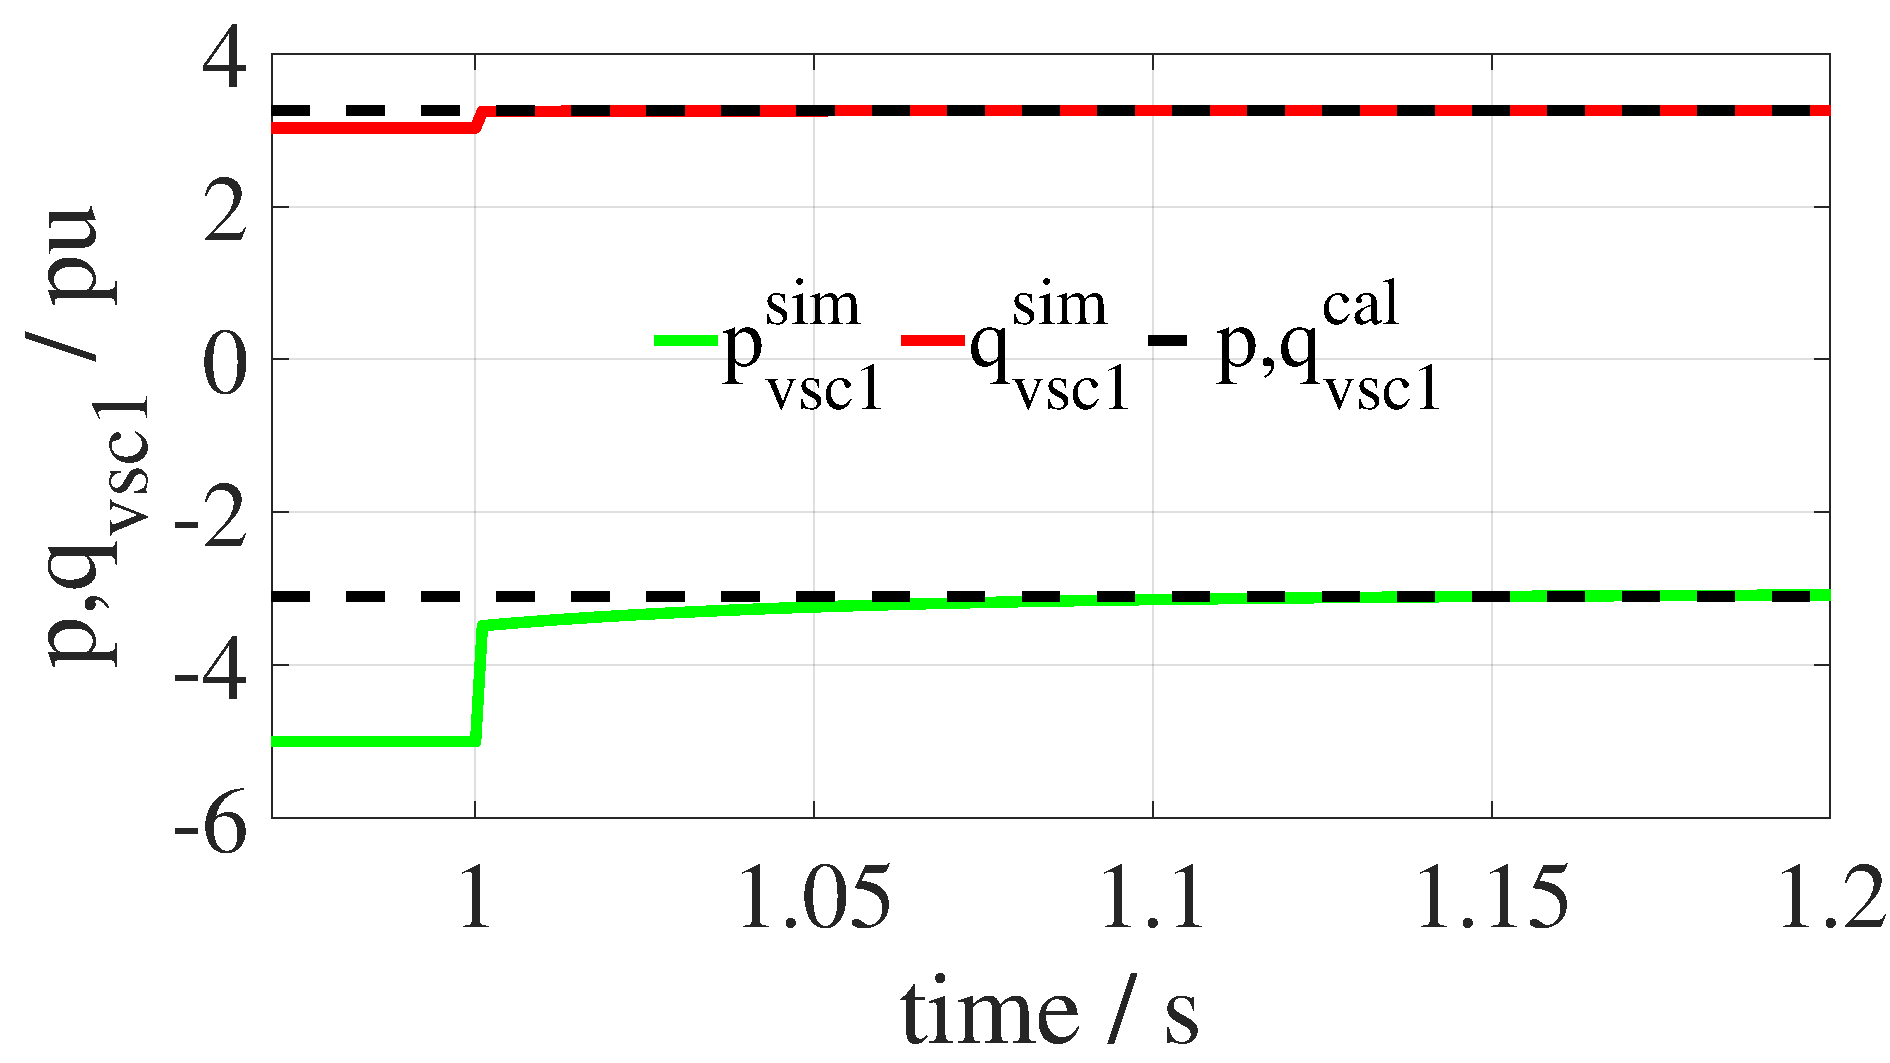
\includegraphics[width=4cm]{Data/Figure/psim_z005.pdf}}
% 	\subfigure[Fault Voltage]{
% 		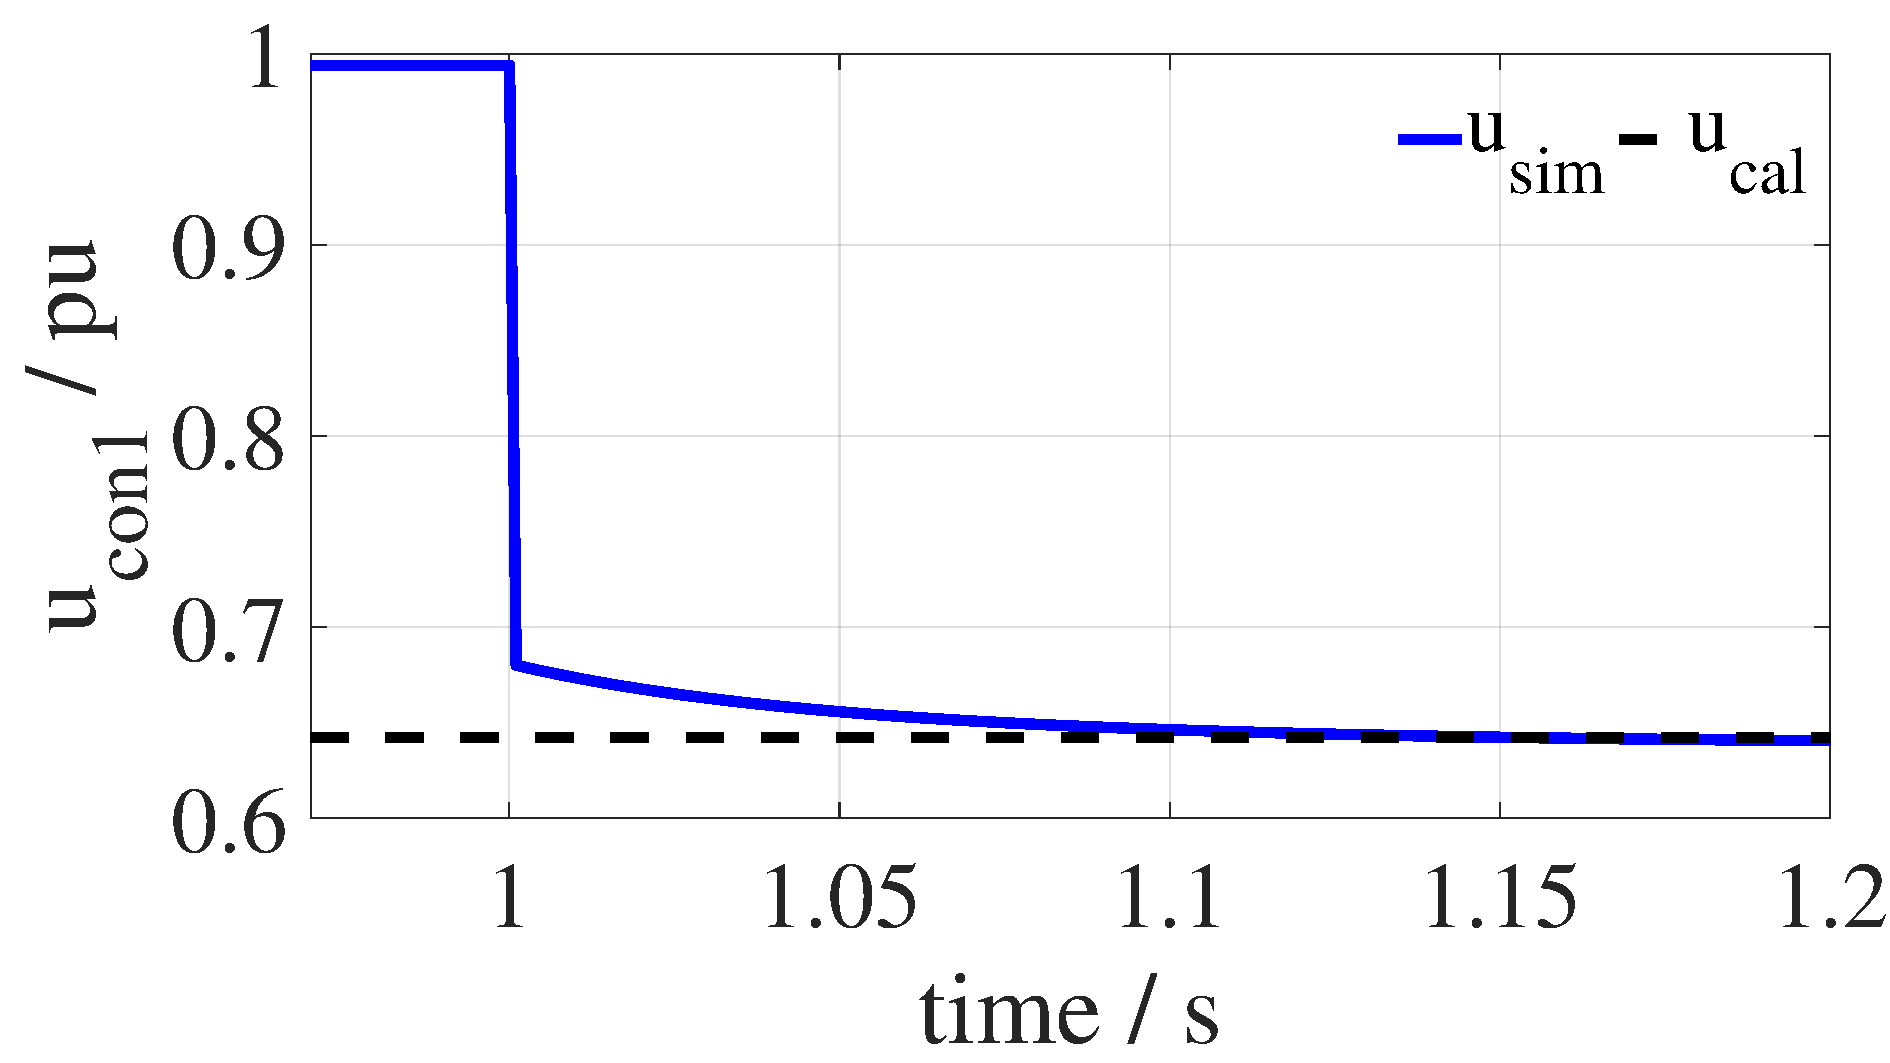
\includegraphics[width=4cm]{Data/Figure/usim_z005.pdf}}
% 	\vskip -2mm
% 	\caption{Moderate Fault with $\underline{z}_{sc}=j0.05$ pu}
% \end{figure}

% \end{frame}






% % \begin{frame}{Results}  % todo more, validated

% % \begin{figure}[!htb]\centering
% % \begin{tikzpicture}
% %   \begin{axis}[axis y line=left, xlabel={Fault impedance (pu)}, ylabel={$I$, $P$, $Q$ (pu)}, grid=both, grid style={line width=.1pt, draw=gray!10}, major grid style={line width=.2pt,draw=gray!50}, xtick distance = 0.05, ytick distance = 0.4, xmin=0.06, xmax=0.50, ymin=0, ymax=3.8, width=11.0cm, height=6.0cm, every plot/.append style={very thick}, very thick, legend style={at={(0.3,0.05)},anchor=south west, legend columns=-1}, y tick label style={/pgf/number format/fixed}, x tick label style={/pgf/number format/.cd, /pgf/number format/fixed, /pgf/number format/precision=3}, scaled x ticks = false, scaled y ticks=false]
% % \addplot[each nth point=1] table[col sep=comma, x=Z, y=I] {Data/vsc2.csv};
% % \addplot[each nth point=1, dashed] table[col sep=comma, x=Z, y=P] {Data/vsc2.csv};
% % \addplot[each nth point=1, gray, dashed] table[col sep=comma, x=Z, y=Q] {Data/vsc2.csv};
% % \legend{$I$, $P$, $Q$};
% % \end{axis}

% %   \begin{axis}[axis y line=right, axis x line=none, ylabel={$V$ (pu)}, major grid style={line width=.2pt,draw=gray!50}, ytick distance = 0.1, width=11.0cm, height=6.0cm, ymin=0.40, ymax=1.3, xmin=0.06, xmax=0.5, every plot/.append style={very thick}, very thick, legend style={at={(0.7,0.05)},anchor=south west, legend columns=-1}, y tick label style={/pgf/number format/fixed}, scaled y ticks=false]
% % \addplot[each nth point=1, gray] table[col sep=comma, x=Z, y=V] {Data/vsc2.csv};
% % \legend{$V$};
% % \end{axis}

% % \draw[thick, fill=orange!60!white] (0,3.7) rectangle (2.1,4.1) node[] (rect) {};
% % \draw[thick, fill=cyan!60!white] (2.1,3.7) rectangle (2.9,4.1) node[] (rect) {};
% % \draw[thick, fill=green!60!white] (2.9,3.7) rectangle (9.42,4.1) node[] (rect) {};

% % % \node at (1.5,3.9) {DIS};
% % \node at (1.05,3.9) {FSS};
% % \node at (2.5,3.9) {PSS};
% % \node at (6.16,3.9) {USS};

% % \end{tikzpicture}
% % \caption{Magnitudes and state depending on the fault impedance for VSC2.}
% %     \label{fig:vsc2}
% % \end{figure}


% % \end{frame}

% \subsection{Computing Efficiency}

% \begin{frame}{Time complexity of our methodology}
%   \begin{itemize}
%     \item As a reference, we should attempt to get a complexity of $\mathcal{O}(n^{1+2\gamma})$.
%     \item Calculating an inverse matrix has in principle a complexity of $\mathcal{O}(n^3)$.
% \end{itemize}
% \begin{equation}
%   - \bm{\Delta f} = \bm{J} \bm{\Delta x}.
% \end{equation}
% Do not calculate $\bm{J}^{-1}$. Rather, use \texttt{scipy.linalg.spsolve}($J, -\Delta f$).

% \begin{table}[!htb]\centering
%   \caption{Average computational time for different systems including converters.}
%   \begin{tabular}{ccc}
%     \hline
%     \textbf{System} & \textbf{Time (ms)} \\
%     \hline
%     \hline
%     IEEE14 & 21.69 \\
%     IEEE39 & 25.52 \\
%     IEEE118 & 32.38 \\
%     Pegase1354 & 69.48 \\
%     ACTIVSg2000 & 82.42 \\
%     \hline
%   \end{tabular}
%   \label{tab:time1}
% \end{table}
% Roughly 14~ms for each iteration in the 2000-bus system.

% \end{frame}

% \begin{frame}{Notes on sparsity}
%   \begin{figure}
%     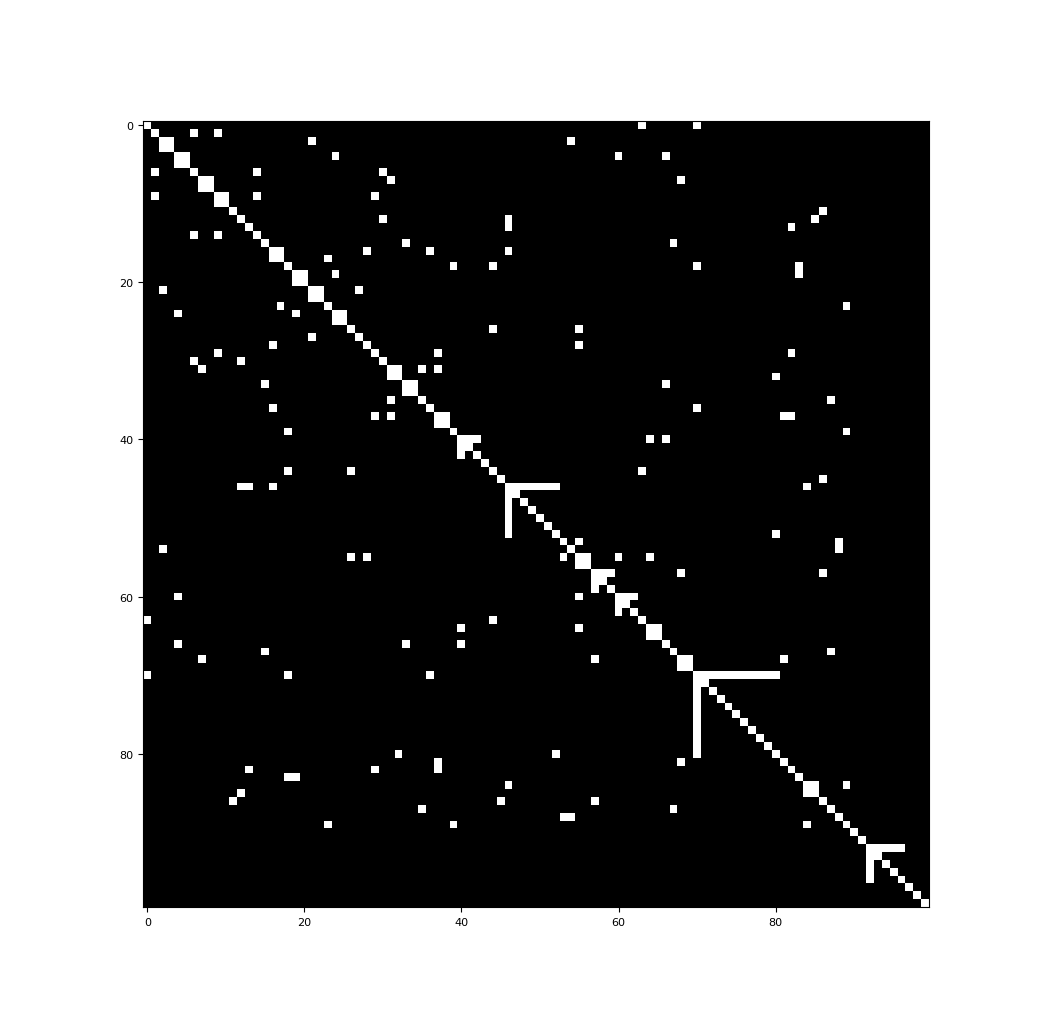
\includegraphics[width=7cm]{Data/jacobian100.png}
%     \caption{First 100 rows and columns for the 2000-bus Jacobian.}
%     \label{fig:jac}
%   \end{figure}
% \end{frame}

% \begin{frame}{Comparison of Computing Efficiency}
% 	When the fault dynamics are dominated by synchronous machines instead of VSCs, longer time is required in order to achieve steady-state during the fault in simulations:
% 	\begin{figure}
% 		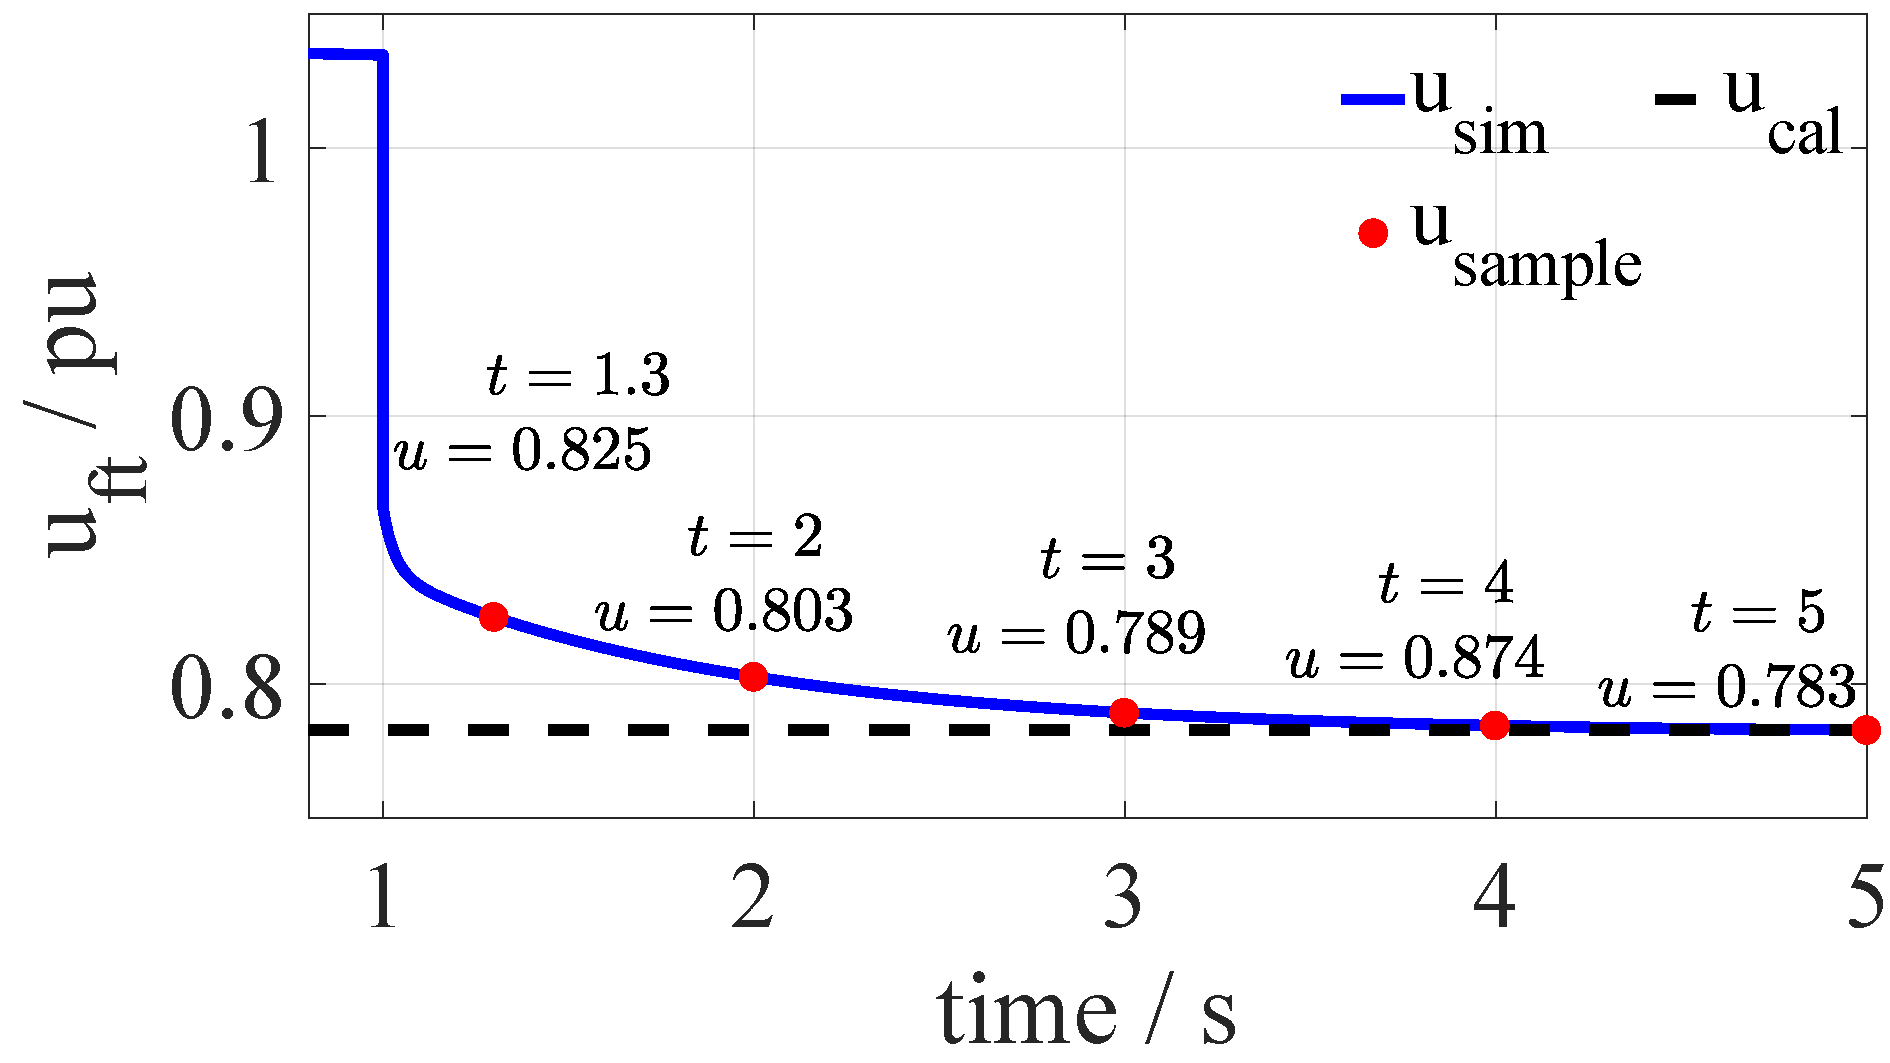
\includegraphics[width=7cm]{Data/Figure/usim_6111.pdf}
% 		\caption{PSSE Simulation With $\underline{z}_{sc}=j0.05$ pu Inserted at Bus 6111.}
% 	\end{figure}
% \end{frame}

% \begin{frame}{Comparison of Computing Efficiency}
% 	The results indicate that our steady-state methodology has advantage in computing time compared to PSSE simulation to achieve the accurate short-circuit calculation results:
% 	\begin{table}[!htb]
%       \renewcommand{\arraystretch}{1.25}
% 		\begin{center}
% 			\caption{Analysis of PSSE Simulation Efficiency*}
% 			\scriptsize
% 			\begin{tabular}{m{3cm}<{\centering}|m{2.5cm}<{\centering}m{4cm}<{\centering}}
% 				\toprule
% 				$t_{sim}$ after fault occurrence & Simulation execution time	& Error $|u_{sample}-u_{cal}|$	\\
% 				\midrule
% 				0.3 s & 1.43 s & $42 \times 10^{-3}$ pu \\
% 				\hline
% 				1 s & 3.52 s & $19.8 \times 10^{-3}$ pu \\
% 				\hline
% 				2 s & 6.81 s & $6.5 \times 10^{-3}$ pu \\
% 				\hline
% 				3 s & 10.07 s & $1.6 \times 10^{-3}$ pu \\
% 				\hline
% 				4 s & 13.14 s & $<0.1 \times 10^{-3}$ pu \\
% 				\hline
%                 \rowcolor[gray]{0.85} Steady-State Calculation & 0.085 s & $6.17 \times 10^{-11}$ pu \\
% 				\bottomrule
% 			\end{tabular}
% 		\end{center}
% 	\end{table}	

% {\scriptsize * Results obtained with $\Delta_t = 1 \times 10^ {-4}$ and $tol = 1 \times 10^ {-4} $ in PSSE simulation.}
	
% \end{frame}

% \begin{frame}{Why should we care about time?}
%   Imagine:
%   \begin{itemize}
%     \item A 2000-bus system with converters.
%     \item A sweep of 10 fault impedances at each bus.
%     \item There is a total of 20000 combinations.
%   \end{itemize}

%   Assuming a dynamic simulation takes $\approx$5~s, and eRoots needs 80~ms:
%   \begin{itemize}
%     \item 1.16 days to complete the dynamic simulation.
%     \item 26.7 minutes to solve with eRoots.
%   \end{itemize}
% \end{frame}

% \subsection{Applications}
% \begin{frame}{Applications}
%   Some applications where time complexity and accuracy become critical are:
%   \begin{itemize}
%     \item Typical power flow with unsaturated VSCs.
%     \item Short-circuit fault with saturated VSCs.
%     \item Fault impedance and location sweeps.
%     \item Variations of VSCs powers to maximize voltage support.
%     \item Assessment of optimal position of VSCs to reduce losses, rise voltages...
%     \item $N-1$ contingency analysis.
%     \item Accurate initialization for dynamics and stability studies.
%   \end{itemize}
% \end{frame}

% \begin{frame}{Novel Grid Equivalent Representation}

% 	\begin{figure}
% 	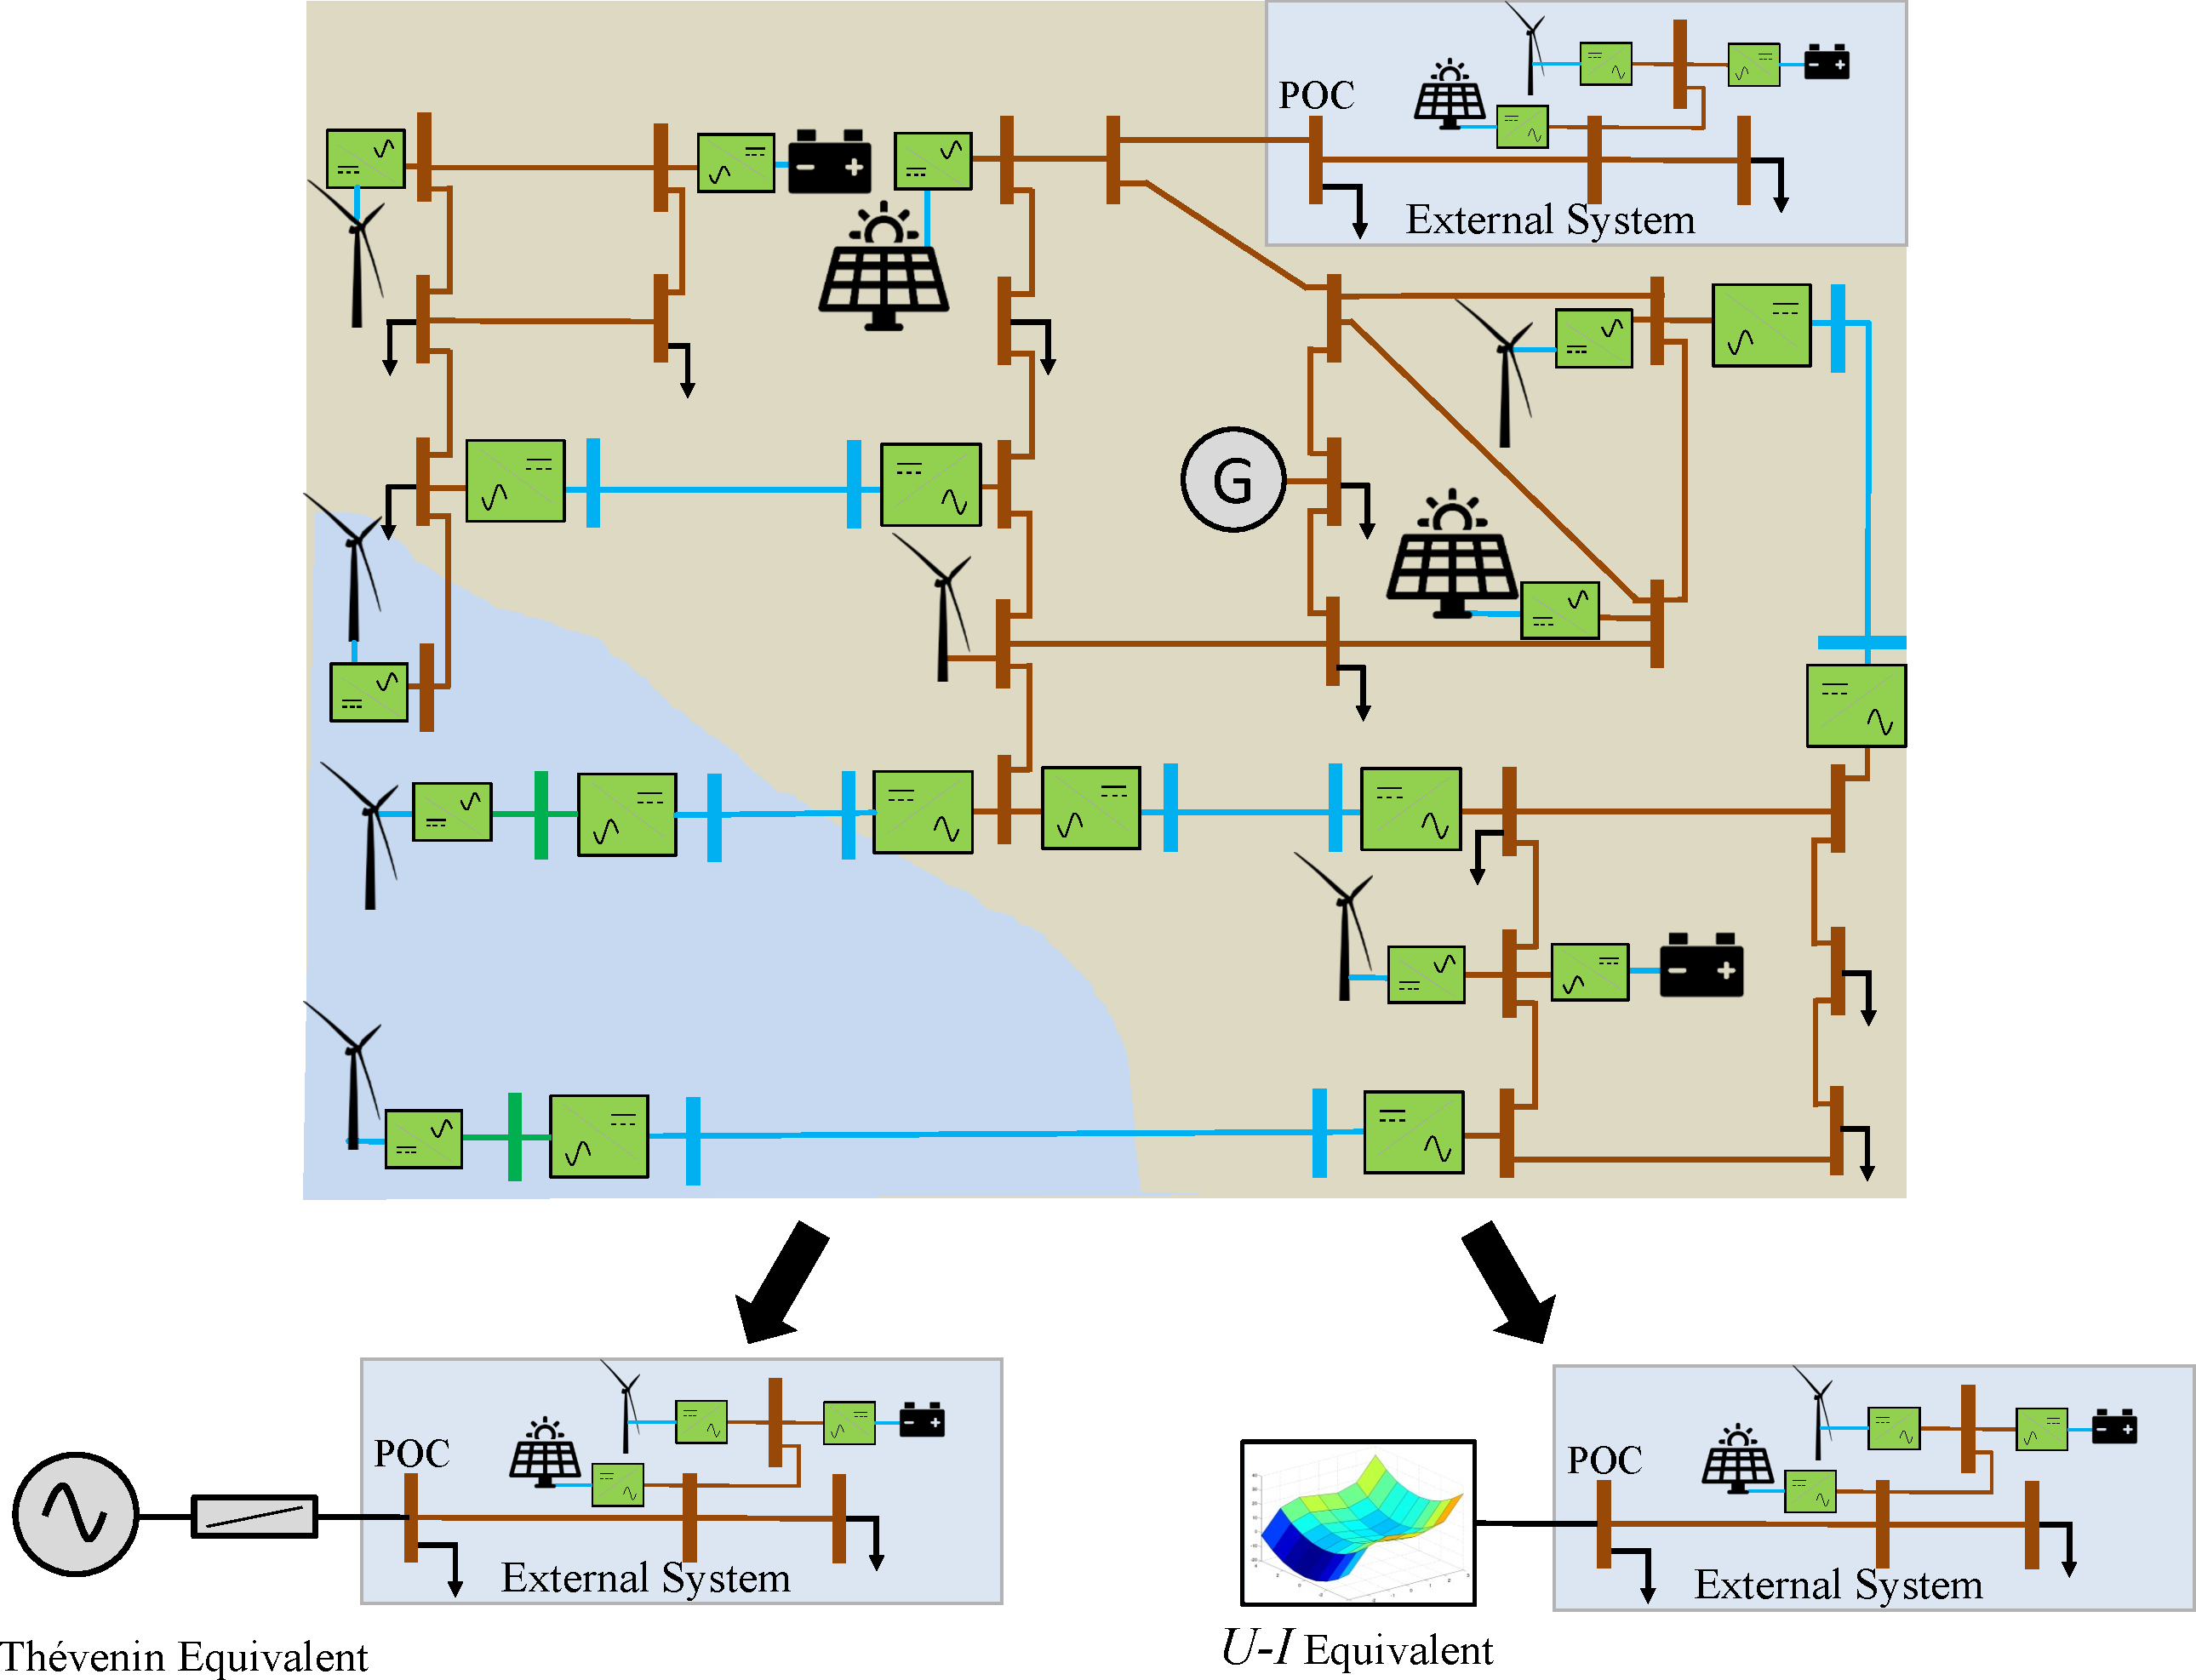
\includegraphics[width=6.5cm]{Data/Figure/Conception.pdf}
% 	\caption{Conception of The Grid Equivalent Representation.}
% 	\end{figure}

% Thévenin equivalent fails to include the non-linear operation of power electronics, a novel grid equivalent representation if proposed as an alternative.

% \end{frame}

% \begin{frame}{Process to Build The \textit{U-I} Equivalent}
	
% Grid equivalent constructed based on voltage-current (\textit{U-I}) characteristics of the studied system from the selected node (point of connection, POC):

%   \begin{itemize}
% 	\item Solve the studied system circuits with several different voltage conditions (magnitudes $\times$ angles) at the POC.\\ \leftthumbsup eRoots tool recommended \rightthumbsup
% 	\item Save each tested POC voltage, $\underline{u}_{out}$, and the corresponding current injection, $\underline{i}_{out}$, into an array, $C_{eq}$.
% 	\item An interpolated function can be obtained from $C_{eq}$ as the equivalent representation of the studied system.
% 	\end{itemize}
% \end{frame}

% \begin{frame}{Case Study}
% Studied system in connection with a VSC in PQ control.
% 	\begin{figure}
% 		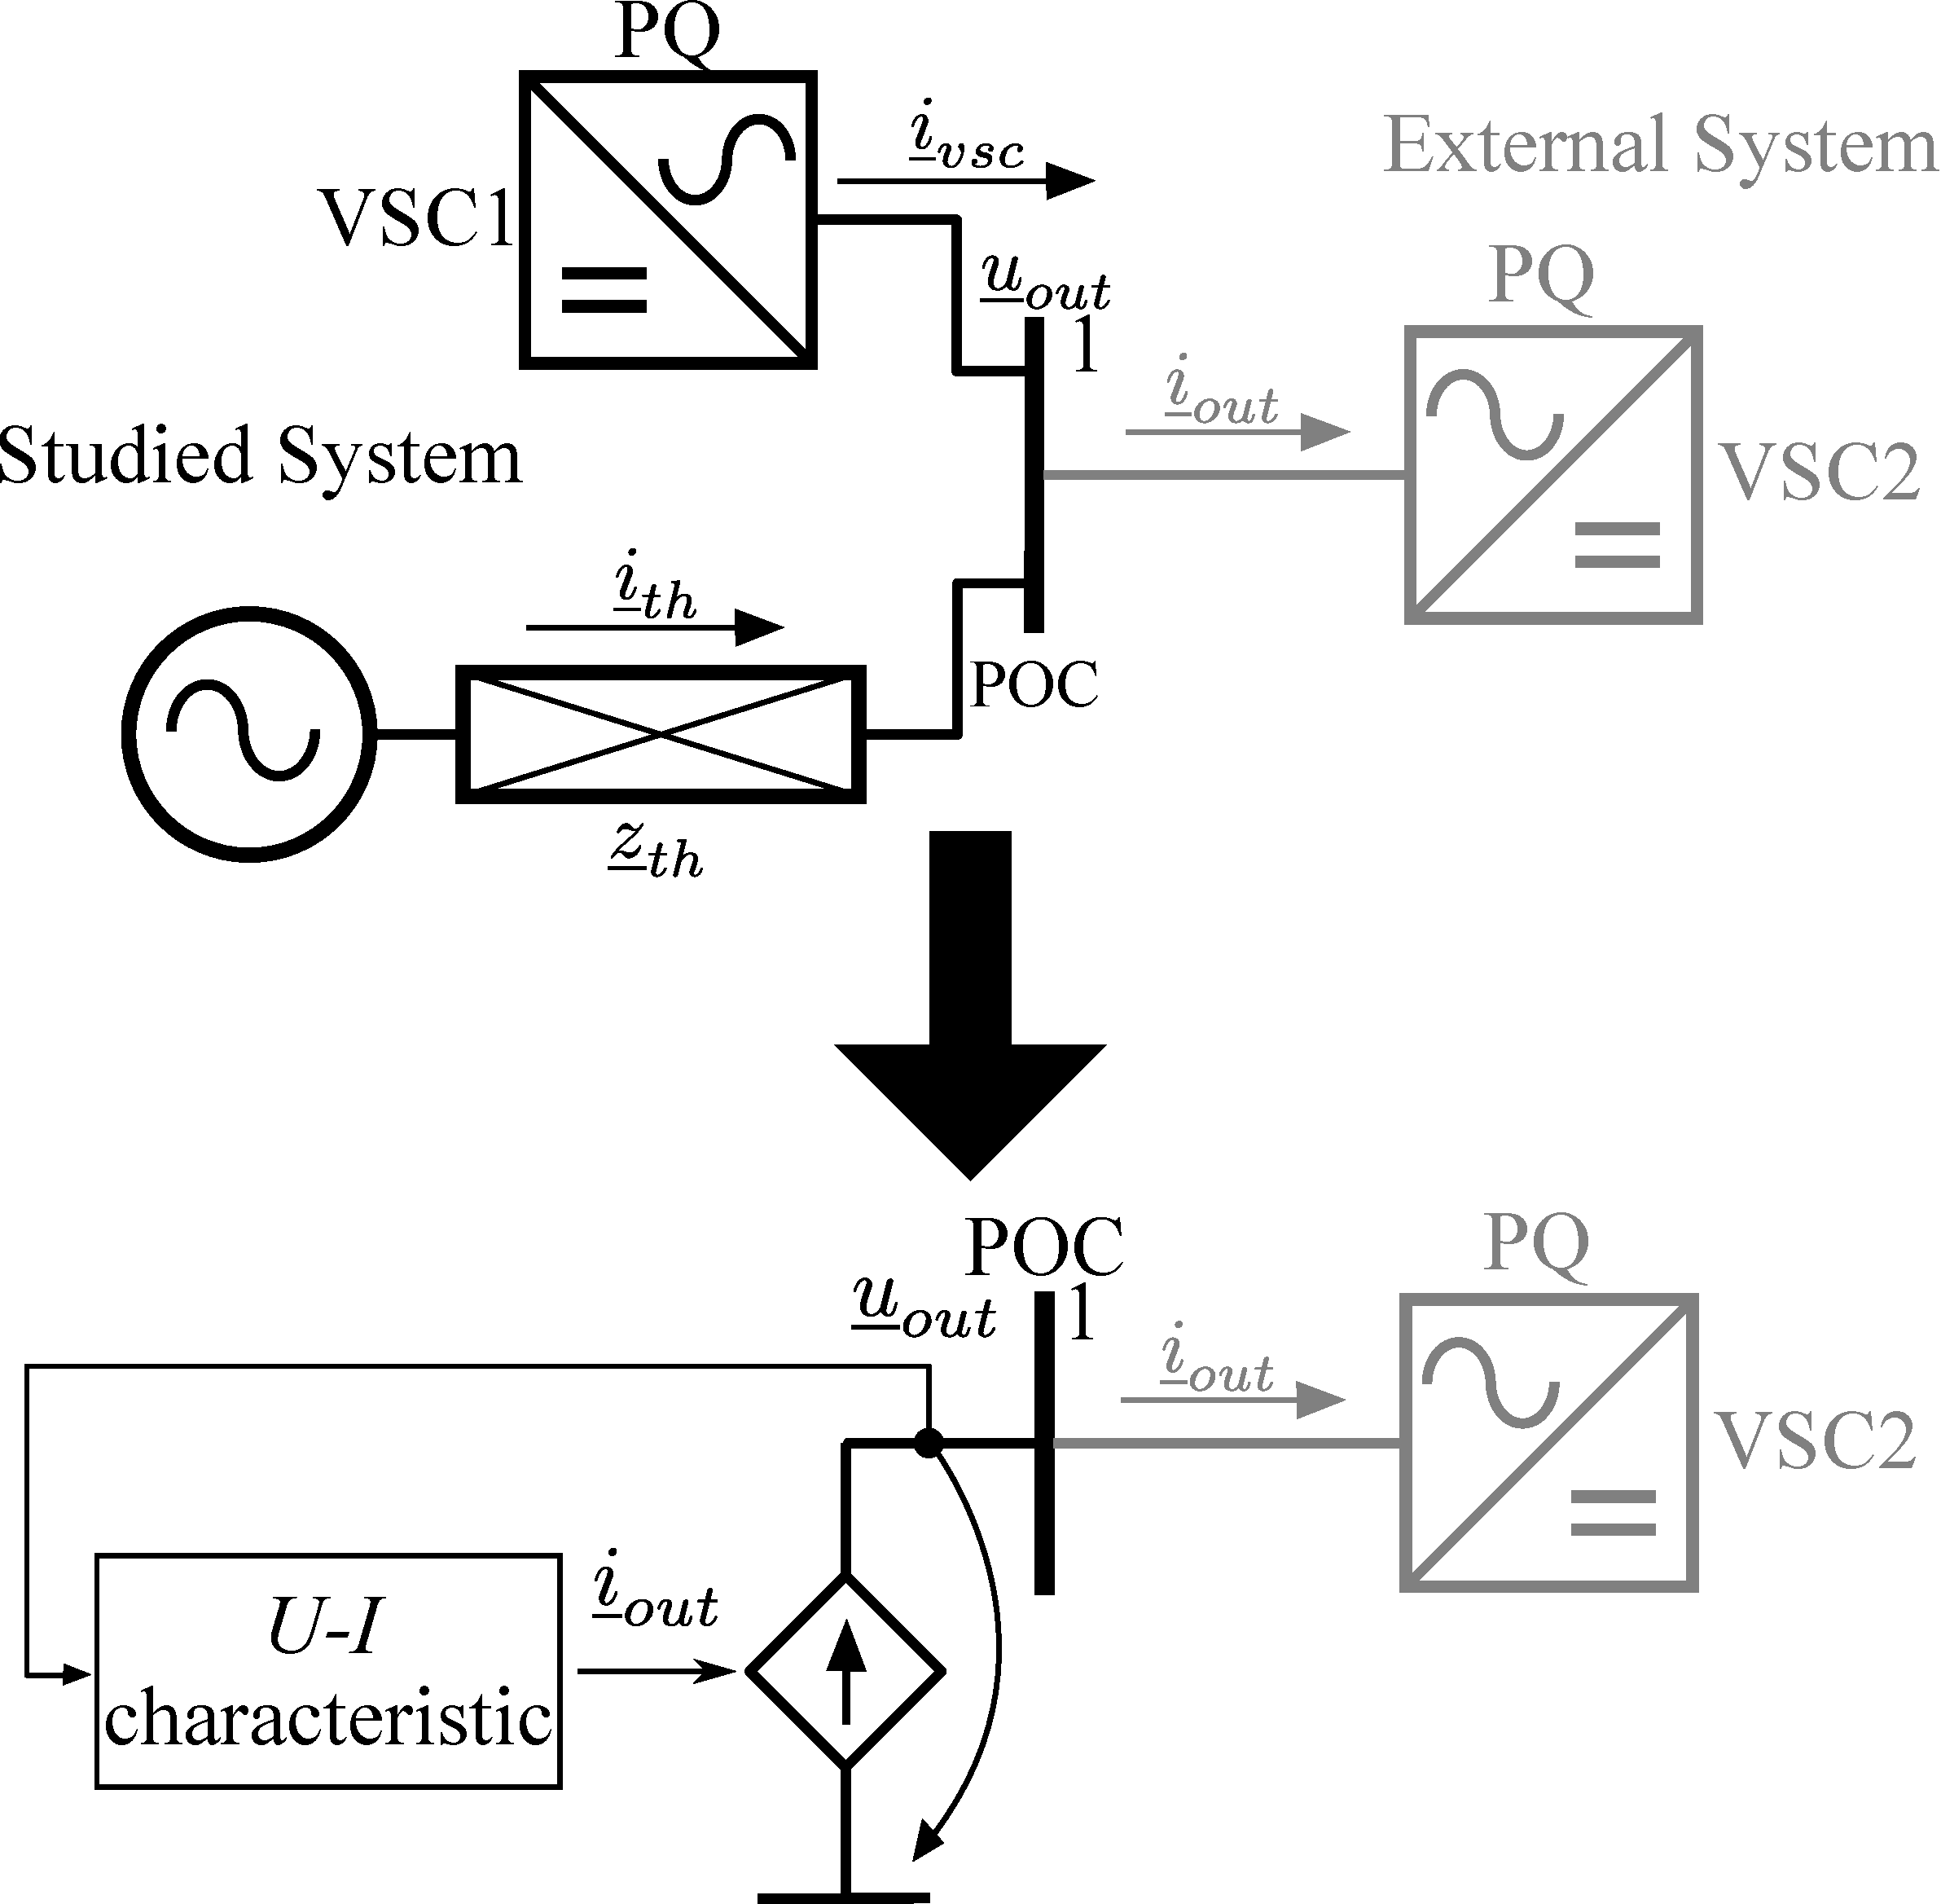
\includegraphics[width=4cm]{Data/Figure/Test1scheme_VSCPQ.pdf}
% 	\end{figure}

% 	\begin{figure}
% 		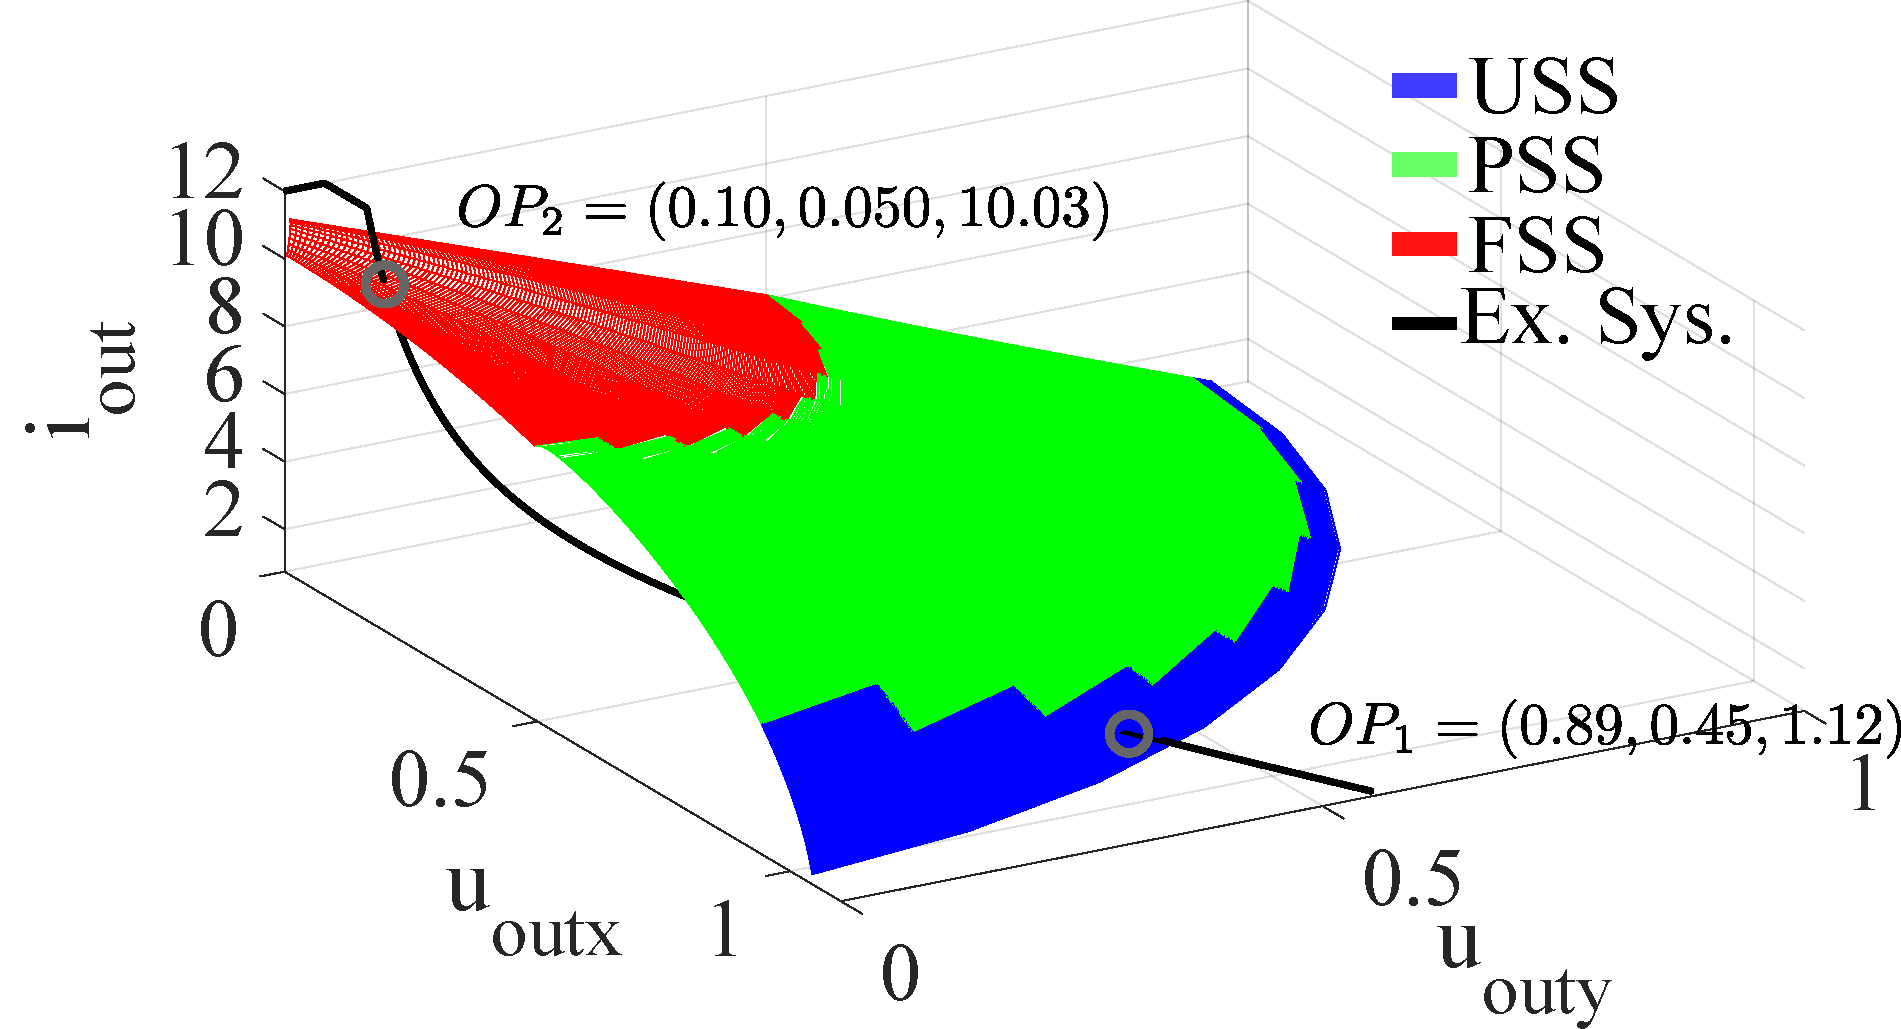
\includegraphics[width=6cm]{Data/Figure/Test1_1.pdf}
% 	\end{figure}
	
% \end{frame}

% \begin{frame}{Case Study}
% 	Short-circuit calculation at the POC.
	
% 	\begin{figure}
% 		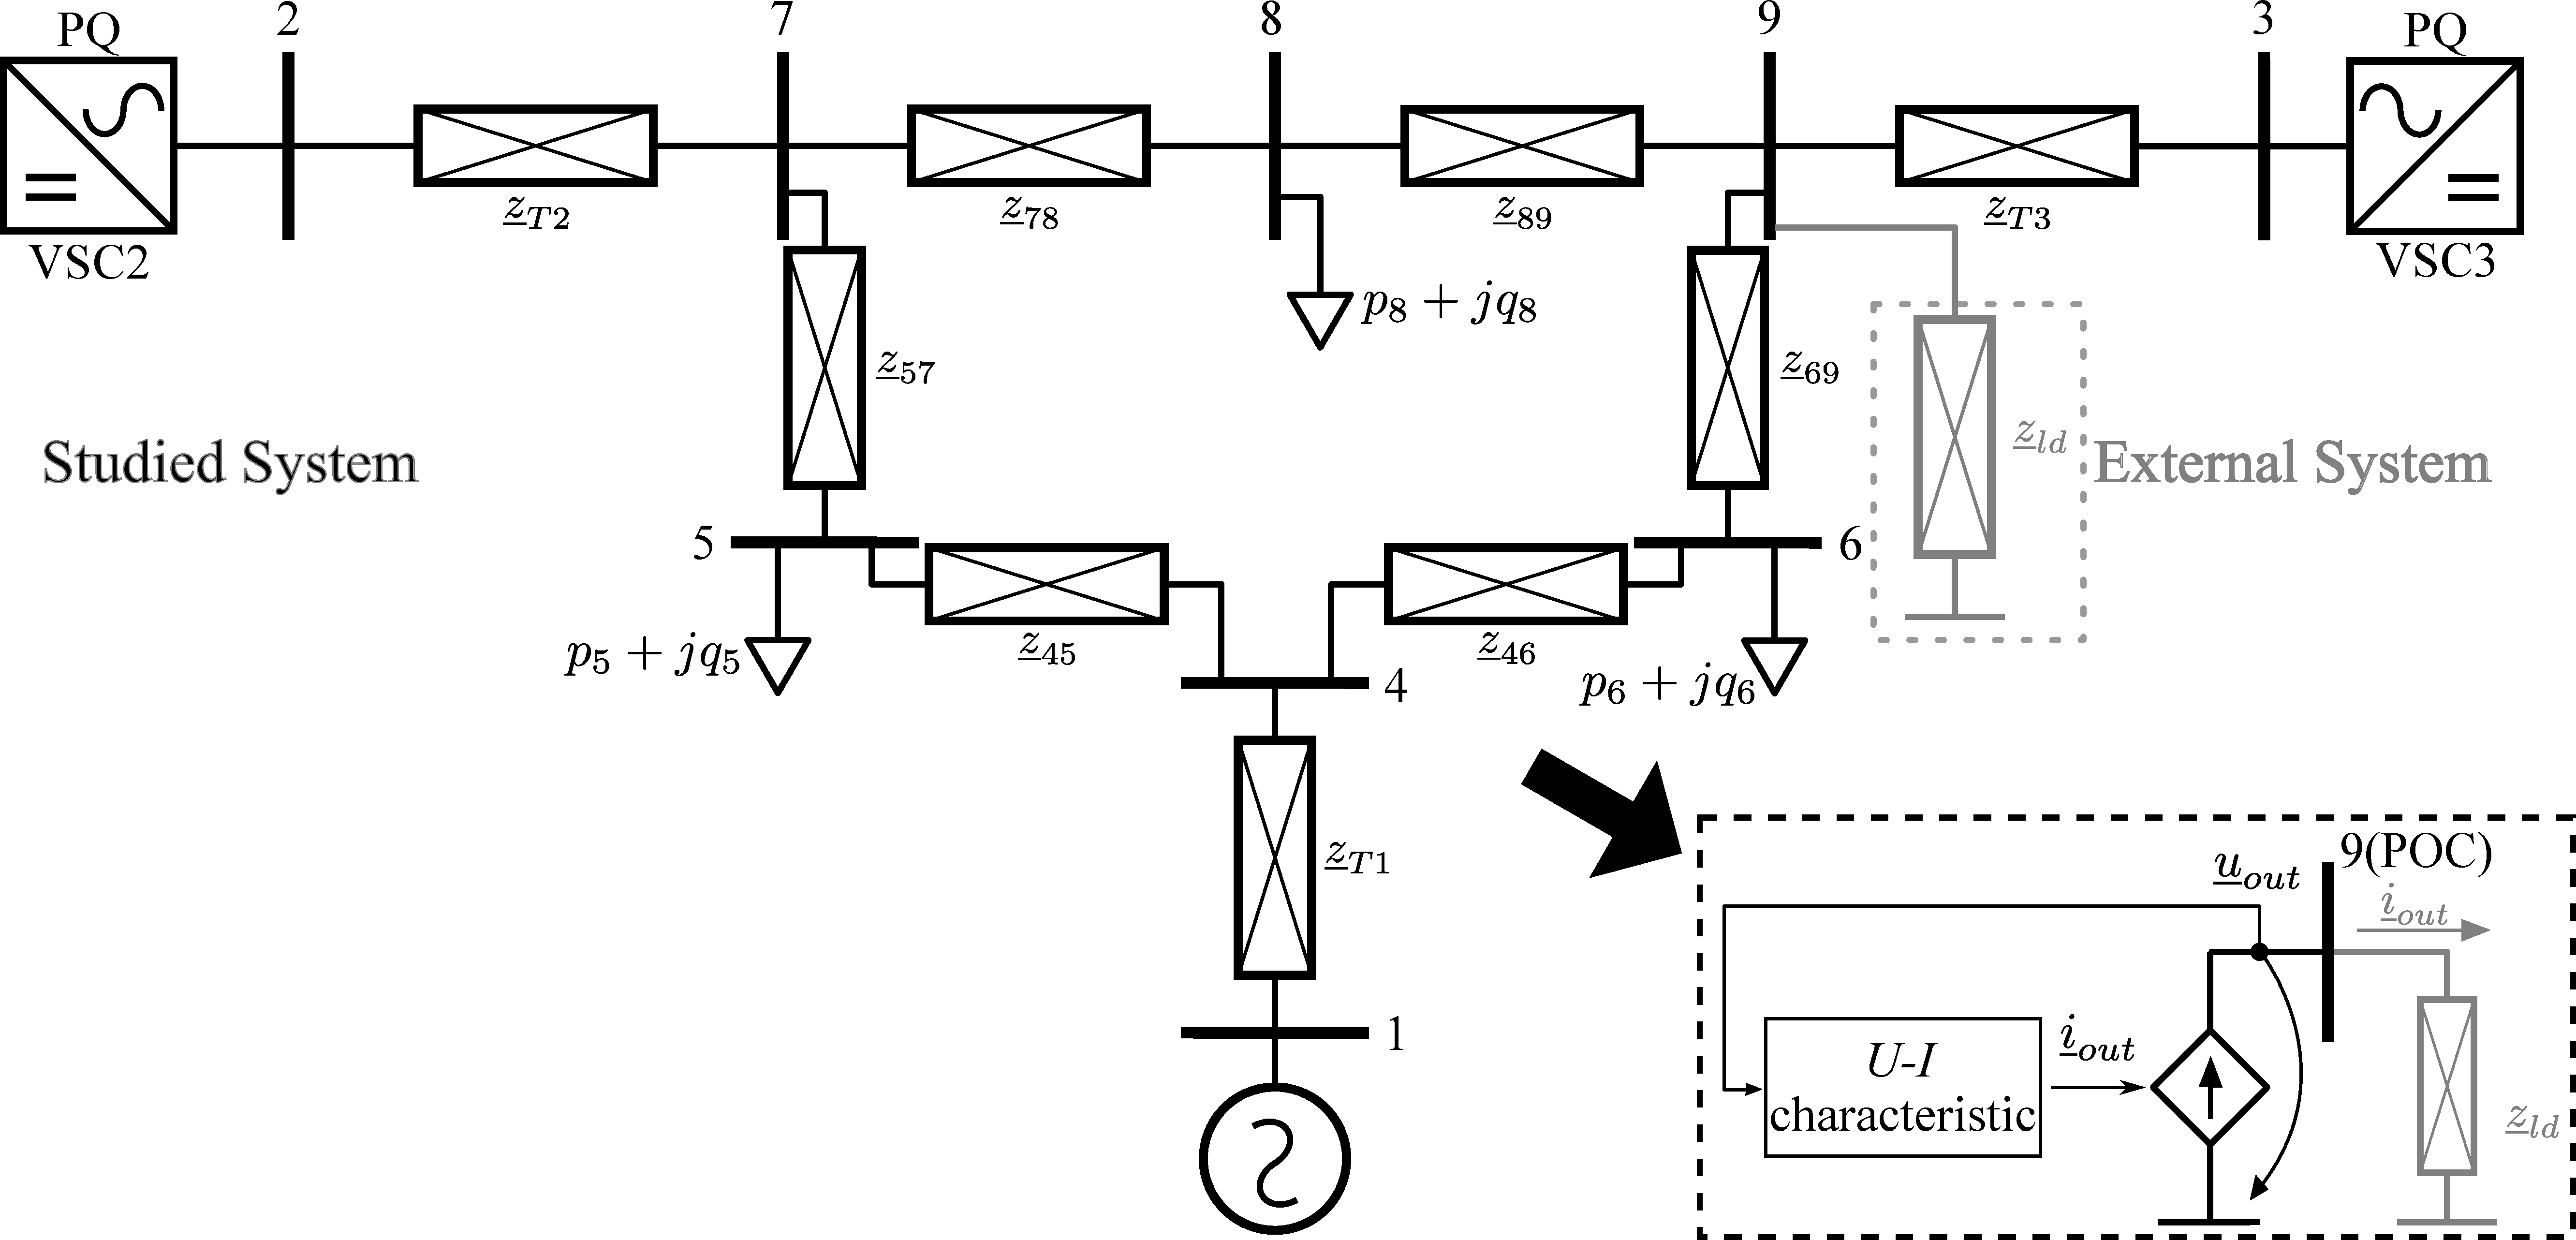
\includegraphics[width=6cm]{Data/Figure/IEEE9_scheme.pdf}
% 	\end{figure}
	
% 	\begin{figure}
% 		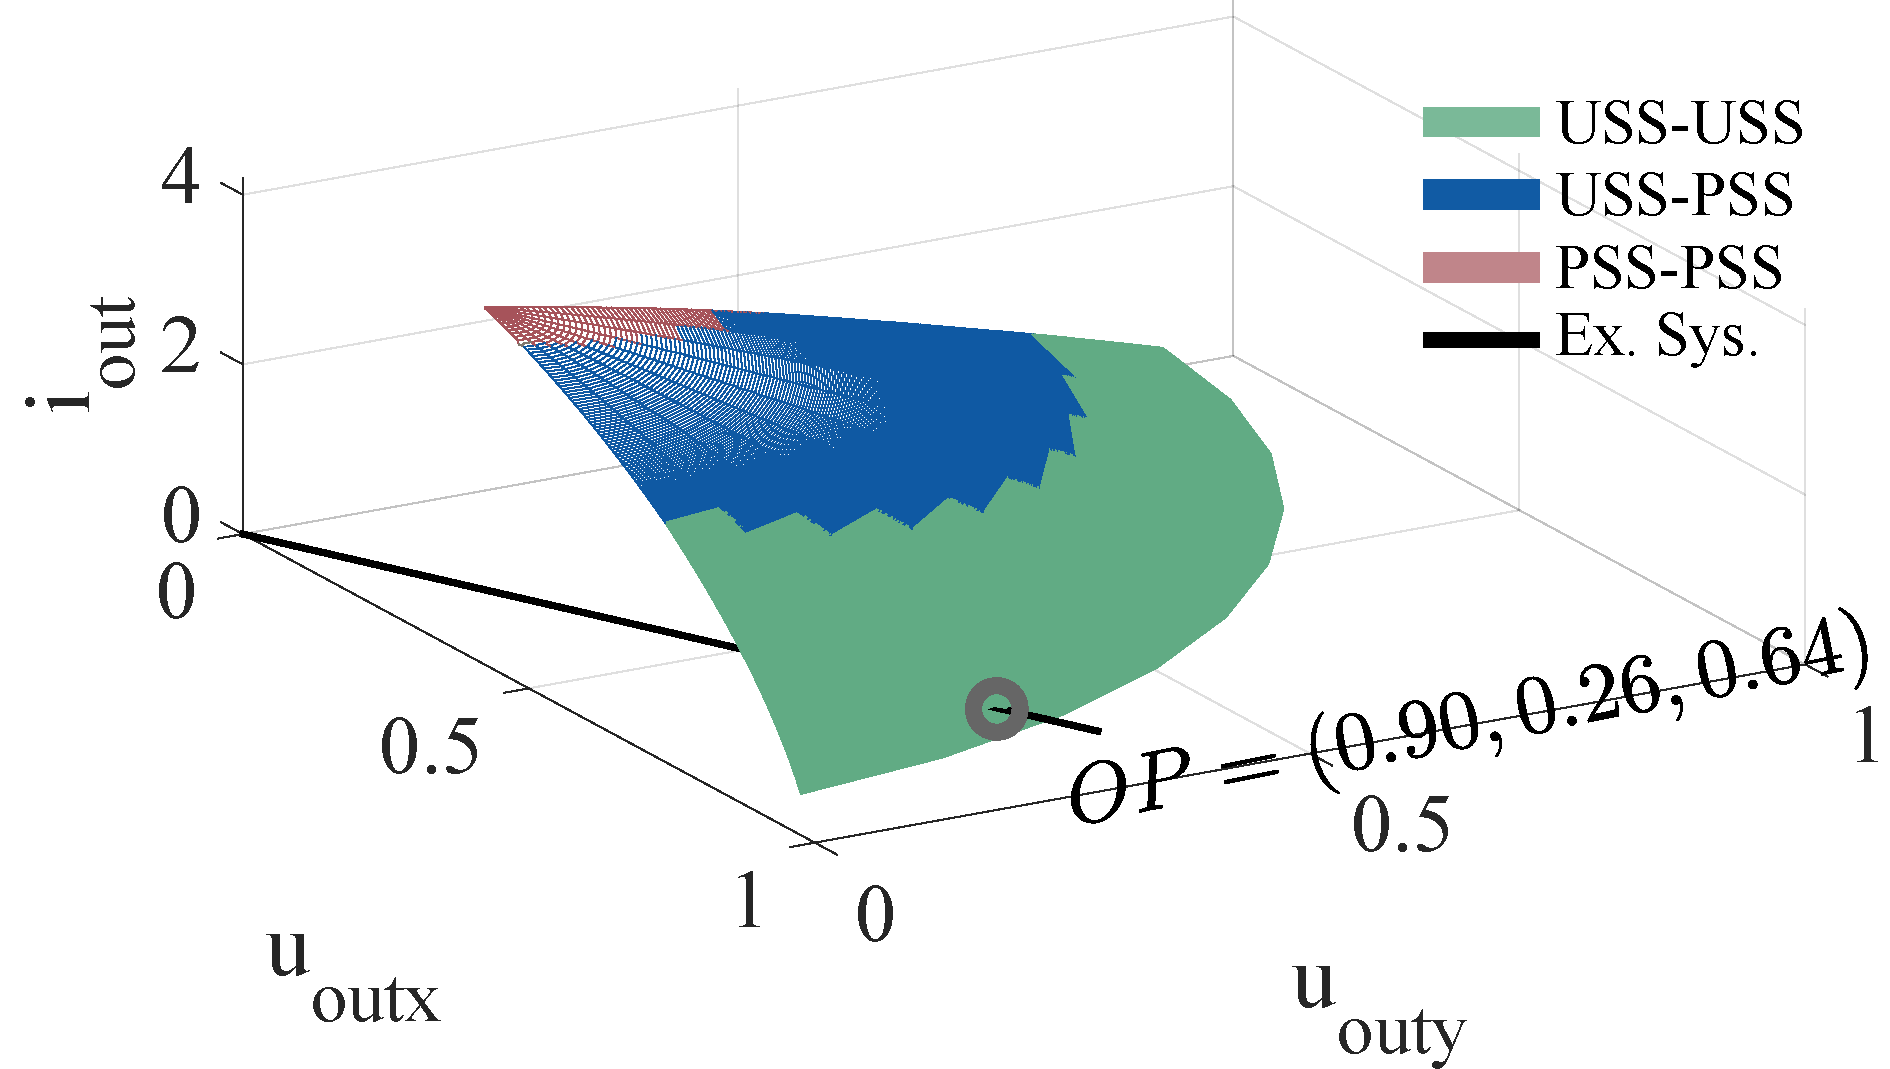
\includegraphics[width=5cm]{Data/Figure/Test2_1.pdf}
% 	\end{figure}
	
% \end{frame}

% \section{Conclusions}
% \begin{frame}{Conclusions}
%   \begin{itemize}
%     \item Adding converters causes the power flow formulation to change.
%     \item Converters can operate in several states. Hence, the type of bus changes. 
%     \item It is mandatory to have a low time complexity.
%     \item Short-circuit faults results have been validated with PSSE simulation.
%   \end{itemize}

% \end{frame}

